%===================================== CHAP 2 =================================

\chapter{Background Theory}

\section{Polarized light}
\label{sec:PolarizedLight} % \text{\color{red}blahblabhbalh plane wave blahblah [short facts, e.g. human's visual range of light]}
Light, in accordance with Maxwell's equations, is described as a propagating electromagnetic (\ac{em}) wave with fundamental properties such as wavelength, intensity and polarization. 

The electric field of a monochromatic plane wave that is completely polarized light and travelling in the $\hat{z}$ direction can be described as a decomposition into two orthogonal field components oscillating in the $\hat{x}$ and $\hat{y}$ directions,
\begin{equation}
    \mathbf{E}(z,t) = E_{0x}\cos(\omega t - kz + \delta_x)\mathbf{\hat{x}} + E_{0y}\cos(\omega t - kz + \delta_y)\mathbf{\hat{y}}
    \label{eq:cosEfield}
\end{equation} 
where $\omega$ and $k$ are the angular frequency and wave vector of the light, while $\delta$ and $E_0$ are phase and amplitude in their respective directions. In complex notation the field is described as
\begin{equation}
    \mathbf{E}(z,t) = E_{0x}e^{i(\omega t - kz + \delta_x)}\mathbf{\hat{x}} + E_{0y}e^{i(\omega t - kz + \delta_y)}\mathbf{\hat{y}},
    \label{eq: Efield}
\end{equation}
where taking the real part of equation (\ref{eq: Efield}) results in the physical field. The magnetic field can be described in a similar manner. However, since the magnetic susceptibility of materials studied in this thesis is comparable to that of vacuum, it is usually sufficient to only account for the electric field. 

Polarization of light is described by the electric field amplitude $E_{0x}$, $E_{0y}$ and phase difference $\delta = \delta_x-\delta_y$. If the two components in equation (\ref{eq: Efield}) have different phases, the oscillating electric field will trace out an ellipse in the plane perpendicular to its direction of propagation. If, for example, $E_{0y}=0$, the electric field will oscillate only in $\hat{x}$-direction and the light is said to be linearly horizontally polarized\cite{collett}. The time dependence in equation (\ref{eq: Efield}), $e^{(i\omega t)}$, is chosen so that in the case of elliptical polarized light, right circular polarization is defined as a clockwise rotation of the electric field when looking towards the source\cite{hauge}.

The polarization of an electromagnetic wave may also be described in complex vector notation by a so-called Jones vector, 
\begin{equation}
    \mathbf{E} = 
    \begin{pmatrix}
        E_{0x}e^{i\delta_x} \\
        E_{0y}e^{i\delta_y} 
    \end{pmatrix}
    =
    \begin{pmatrix}
        E_{x} \\
        E_{y} 
    \end{pmatrix},
    %\cdot e^{i(\omega t - kz)}
    \label{eq:Jonesvector}
\end{equation}
where the propagator $\omega t - kz$ is usually suppressed when only polarization is of interest\cite{collett}. Again, restoring the propagator and taking the real part of equation (\ref{eq:Jonesvector}) will result in the optical field. The total intensity of the optical field averaged over time is given by
\begin{equation}
    I = E_xE_x^* + E_yE_y^*.
\end{equation}
When describing the change of polarization of light after interaction with an optical element, e.g. reflection from a thin film, a Jones Matrix formulation may be used when assuming a linear relation between the components of the emerging beam and the incident beam,
\begin{equation}
    \begin{pmatrix}
        E_{x} \\
        E_{y} 
    \end{pmatrix}_{out}
    =
    \begin{pmatrix}
        j_{11} & j_{12} \\
        j_{21} & j_{22} 
    \end{pmatrix}
    \begin{pmatrix}
        E_{x} \\
        E_{y} 
    \end{pmatrix}_{inc}
\end{equation}
where the 2x2 matrix is called the Jones Matrix and its elements $j_{kl}\quad(k,l = 1,2)$ are complex reflection or transmission coefficients translating linear interactions of completely polarized light. Reflectance or transmittance, which is the fraction of incident electromagnetic power that is reflected or transmitted by the optical element, is given by $J_{kl} = \abs{j_{kl}}^2$.

\section{Stokes-Mueller formalism}
The Jones formalism provides a description of completely polarized light. However, often in nature and practical cases, light is not a perfectly monochromatic wave\footnote{A wave is monochromatic if amplitude and phase factors are constant for all time, as in section \ref{sec:PolarizedLight}.}. Sunlight, for example, is unpolarized light, meaning that the beam's polarization changes so quickly and randomly that it cannot be determined for any practical purposes. Real-world measurement systems and samples may cause a fraction of the light to become unpolarized. This process where the light's degree of polarization is reduced is called \emph{depolarization}, and describes the percentage of light that has become unpolarized\cite{hans_arwin}. Another limitation of the Jones formalism regarding experimental work is that detectors measure light intensities, not field amplitudes. There is thus a practical motivation for an alternative representation of light in terms of intensities which also takes into account depolarization.

The Stokes-Mueller formalism may represent quasi-monochromatic light that is unpolarized, partially polarized or completely polarized. A quasi-monochromatic wave will have time-dependent phase factors $\delta_i(t)$ and amplitude $E_i(t)$ that fluctuate slowly compared to the rapid oscillations of the cosinusoids in equation (\ref{eq:cosEfield}) \cite{collett}.The Stokes vector provide a full description of any polarization state\cite{azzam},
\begin{equation}
    \begin{pmatrix}
        S_0 \\
        S_1 \\
        S_2 \\
        S_3
    \end{pmatrix}
    =
    \begin{pmatrix}
        <E_{0x}(t)^2> + <E_{0y}(t)^2> \\
        <E_{0x}(t)^2> - <E_{0y}(t)^2> \\
        2<E_{0x}(t)E_{0y}(t)\cos[\delta_y(t) - \delta_x(t)]> \\
        2<E_{0x}(t)E_{0y}(t)\sin[\delta_y(t) - \delta_x(t)]>
    \end{pmatrix}
    =
    \begin{pmatrix}
        I_x + I_y \\
        I_x - I_y \\
        I_{+45\degree} - I_{-45\degree} \\
        I_r - I_l
    \end{pmatrix},
    \label{eq:StokesVector}
\end{equation}
where $<...>$ denotes the time-average, so that $S_0$ represents the total intensity of the light beam, $S_1$ is the intensity difference between horizontally and vertically polarized light, and $S_2$ the difference between $+45\degree$ and $-45\degree$ polarized light. Finally $S_3$ is the difference between right handed and left handed circularly polarized light.
Whereas the Jones vector represent light with field amplitude and phase, the Stokes vector represent light with field intensities. %$I_{x,y}$ is the intensity of linearly polarized light in $\hat{x}$ and $\hat{y}$ directions, 

The degree of polarization $P$ is defined as the ratio between the intensity of completely polarized light to the total intensity of the beam. In terms of Stokes parameters this is 
\begin{equation}
    P = \frac{\sqrt{S_1^2 + S_2^2 + S_3^2}}{S_0}.
\end{equation}
The value $P=1$ corresponds to completely polarized light, $P=0$ corresponds to unpolarized light, and $0<P<1$ corresponds to partially polarized light.

A change in polarization state, from one Stokes vector to another, due to interaction with an optical element is expressed through the matrix equation $\mathbf{S}_{out} = \mathbf{M}\mathbf{S}_{inc}$, where $\mathbf{M}$ is a 4x4 matrix called the Mueller matrix (\ac{mm}) of the system. Written out in terms of the elements, this becomes
\begin{equation}
    \begin{pmatrix}
        S_0 \\
        S_1 \\
        S_2 \\
        S_3
    \end{pmatrix}_{out}
    =
    \begin{pmatrix}
    M_{11} & M_{12} & M_{13} & M_{14}   \\
    M_{21} & M_{22} & M_{23} & M_{24}   \\
    M_{31} & M_{32} & M_{33} & M_{34}   \\
    M_{41} & M_{42} & M_{43} & M_{44}   \\
    \end{pmatrix}
    \begin{pmatrix}
        S_0 \\
        S_1 \\
        S_2 \\
        S_3
    \end{pmatrix}_{inc},
\end{equation}
where the elements are real numbers that may take values $M_{ij}\in[-1,1]$. The MM describes the optical element, and contains all the information about what happens to the polarization state during the interaction. The polarization state may be changed by changing the orthogonal field amplitudes unequally (diattenuation), changing the phase (retardance), changing the direction of the orthogonal field components (rotation), or transferring energy from polarized states to unpolarized states (depolarization). Any system's MM may be deconstructed into a succession of optical components, each described by its own MM, i.e.\cite{hans_arwin}
\begin{equation}
    \mathbf{M} = \mathbf{M}_N \mathbf{M}_{N-1}...\mathbf{M}_1, 
\end{equation}
where light propagates from 1 to $N$.

If the optical system is non-depolarizing, the MM may be fully described by a Jones matrix. For such a system described by the Jones matrix $\mathbf{J}$, the corresponding Mueller matrix is given by \cite{hans_arwin}
\begin{equation}
    \mathbf{M} = \mathbf{A}(\mathbf{J}\otimes\mathbf{J}^*)\mathbf{A}^{-1}
    \label{eq:JonesMuellerConversion}
\end{equation}
where $\otimes$ is the Kronecker product and 
\begin{equation}
    \mathbf{A} = 
    \begin{pmatrix}
        1 & 0 & 0 & 1 \\
        1 & 0 & 0 & -1 \\
        0 & 1 & 1 & 0 \\
        0 & i & -i & 0
    \end{pmatrix}.
\end{equation}
In the case of reflection off a non-depolarizing sample, in a coordinate system defined by the beam's plane of incidence (\ac{poi}) where the electric field orthogonal components are directed either parallel to POI (p-polarization) or perpendicular to the POI (s-polarization), the general reflection Jones matrix is
\begin{equation}
    \mathbf{r} = 
    \begin{pmatrix}
        r_{pp}  &   r_{ps}  \\
        r_{sp}  &   r_{ss}  \\
    \end{pmatrix},
    \label{eq:reflectionJonesMatrix}
\end{equation} % the portion of the incident beam that initially was $\beta$-polarized is converted to $\alpha$-polarization after reflection.
see figure \ref{fig:principle_of_ellipsometry}. The matrix elements in equation (\ref{eq:reflectionJonesMatrix}) are complex reflection coefficients. The convention of subscript notation is here used such that $r_{\alpha\beta}$ indicates the portion of the initially $\beta$-polarized wave that is converted to $\alpha$-polarization after reflection. The off-diagonal elements therefore describe conversion between the two polarization modes. Conversion equations for the equivalent MM \cite{hauge}, found by inserting the reflection Jones matrix (\ref{eq:reflectionJonesMatrix}) into equation (\ref{eq:JonesMuellerConversion}), are listed below
\begin{subequations}
\begin{align}
    M_{11} &= \frac{1}{2}(\abs{r_{pp}}^2 + \abs{r_{ps}}^2 + \abs{r_{sp}}^2 + \abs{r_{ss}}^2)    \\
    M_{12} &= \frac{1}{2}(\abs{r_{pp}}^2 - \abs{r_{ps}}^2 + \abs{r_{sp}}^2 - \abs{r_{ss}}^2)     \\
    M_{13} &= \text{Re}[r_{pp}r_{ps}^* + r_{sp}r_{ss}^*]    \\
    M_{14} &= \text{Im}[r_{pp}r_{ps}^* + r_{sp}r_{ss}^*]    \\
    M_{21} &= \frac{1}{2}(\abs{r_{pp}}^2 + \abs{r_{ps}}^2 - \abs{r_{sp}}^2 - \abs{r_{ss}}^2)     \\
    M_{22} &= \frac{1}{2}(\abs{r_{pp}}^2 - \abs{r_{ps}}^2 - \abs{r_{sp}}^2 + \abs{r_{ss}}^2)     \\
    M_{23} &= \text{Re}[r_{pp}r_{ps}^* - r_{sp}r_{ss}^*]    \\
    M_{24} &= \text{Im}[r_{pp}r_{ps}^* - r_{sp}r_{ss}^*]    \\
    M_{31} &= \text{Re}[r_{pp}r_{sp}^* + r_{ps}r_{ss}^*]    \\
    M_{32} &= \text{Re}[r_{pp}r_{sp}^* - r_{ps}r_{ss}^*]    \\
    M_{33} &= \text{Re}[r_{pp}r_{ss}^* + r_{ps}r_{sp}^*]    \\
    M_{34} &= \text{Im}[r_{pp}r_{ss}^* - r_{ps}r_{sp}^*]    \\
    M_{41} &= -\text{Im}[r_{pp}r_{ps}^* + r_{sp}r_{ss}^*]    \\
    M_{42} &= -\text{Im}[r_{pp}r_{ps}^* - r_{sp}r_{ss}^*]    \\
    M_{43} &= -\text{Im}[r_{pp}r_{ss}^* + r_{ps}r_{sp}^*]    \\
    M_{44} &= \text{Re}[r_{pp}r_{ss}^* - r_{ps}r_{sp}^*].    \\
\end{align}
    \label{eq:JonesToMueller}
\end{subequations}
Note that there is a clear indication of polarization coupling induced by the sample if the off-diagonal block elements are non-zero.

\begin{figure}
    \centering
    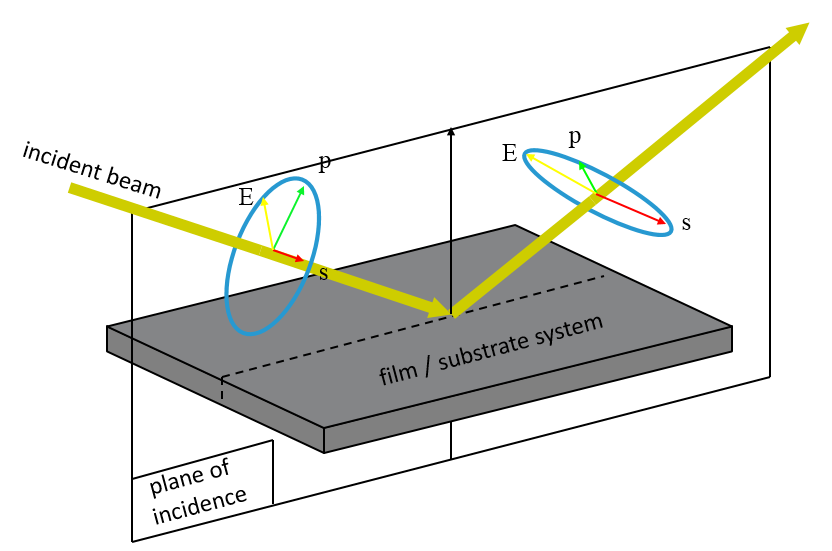
\includegraphics[scale=0.75]{figures/Ch2/principle_of_ellipsometry.png}
    \caption{Light reflected at the interface between two media. Direction of electric field is defined from the beam's plane of incidence as p-polarization and s-polarization. Source \cite{ellipsometry_fig}.}
    \label{fig:principle_of_ellipsometry}
\end{figure}

There are many necessary conditions that must be met for a MM to be physically realizable\cite{hans_arwin}\cite{realizableMM}. Here, however, the subject will only be briefly discussed. The question is which conditions should be imposed on the elements of $\mathbf{M}$ in order for it to correspond to a real physical system. Consider the optical system in figure \ref{fig:principle_of_ellipsometry}. The emerging light, i.e. the resulting Stokes vector $\mathbf{S}_{out}$ after the incident light $\mathbf{S}_{inc}$ is operated on by $\mathbf{M}$, cannot have a degree of polarization larger than one and its total intensity must be positive. In other words, it must hold that $S_0^2 \geq S_1^2+S_2^2+S_3^2$ and $S_0 \geq 0$. What are the conditions on a given MM that will ensure that the output light is partially polarized for any polarization of the input light, or equivalently, when will the degree of polarization $P$ of the output Stokes vector satisfy $P\leq1$ for any physical input Stokes vector? This is a non-trivial matter and many constraints have been derived\cite{realizableMM}\cite{Kostinski:93}. The constraints may even be used for calibration of polarimetric instruments, estimation of experimental errors, and testing computational procedures.

\section{Ellipsometry}
Ellipsometry is an experimental technique for investigating optical properties of thin films and surfaces. It is a form of polarimetry, which is to measure and interpret the polarization state of light. The basic principle of ellipsometry is to measure the change in phase and amplitude of two orthogonal electric field components after it has reflected or transmitted at the sample of interest, see figure \ref{fig:principle_of_ellipsometry}. However, for most samples, an analytic inversion of the ellipsometric equations (discussed in the next section) is not possible and thus the unknown parameters cannot be obtained directly. Instead, a model can be created to calculate a response which is compared to the experimental response. Using regression analysis, fit parameters of the model are adjusted to find a minimum between the model data and experimental data. If the results of the assumed model are not fully in agreement with the experimental data, one may go back and redefine its properties e.g. by adding a roughness layer, anisotropy or graded optical properties. This is repeated until a satisfactory fit is found. How good a fit is can be quantified by a mean-square error or another error function. Figure \ref{fig:ellipsometryOverview} presents an overview of this process\cite{JAWoolam_DataAnalysis}.

Thus, ellipsometry is an indirect method of retrieving optical properties from a sample, such as its dielectric function or refractive index, thin film thickness, surface roughness and layer composition.
\begin{figure}
    \centering
    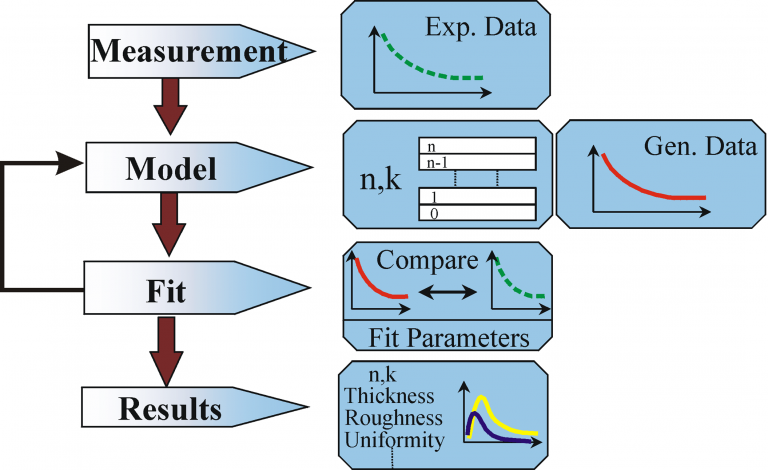
\includegraphics[scale=0.35]{figures/Ch2/EllipsometryOverview.png}
    \caption{Overview of the fit procedure in ellipsometric data analysis. Source \cite{JAWoolam_DataAnalysis}}
    \label{fig:ellipsometryOverview}
\end{figure}

\subsection{Various forms of ellipsometry}
There are mainly three types of ellipsometry, namely standard, generalized and Mueller-matrix ellipsometry. While the methods are here explained in terms of reflection off a sample, the principle and derivation are similar for transmission ellipsometry\cite{handbook_ellipsometry_ch1}.

\subsubsection{Standard ellipsometry}
In standard ellipsometry, a single measurement of the sample-induced change in polarization is performed per wavelength, while assuming no coupling between p- and s-polarization. The reflection Jones matrix, equation (\ref{eq:reflectionJonesMatrix}), is therefore diagonal, the sample reflection properties entirely given by $r_{ss}$ and $r_{pp}$. For light reflected at the interface between two isotropic media 0 and 1 as in figure \ref{fig:SE}, the complex reflection coefficients are the Fresnel equations\cite{azzam}
\begin{subequations}
\begin{align}
    r_{pp} &= \frac{N_1\cos\theta_0 - N_0\cos\theta_1}{N_1\cos\theta_0 + N_0\cos\theta_1}    \\
    r_{ss} &= \frac{N_0\cos\theta_0 - N_1\cos\theta_1}{N_0\cos\theta_0 + N_1\cos\theta_1}
\end{align}
\label{eq:Fresnel_refl_coeff}
\end{subequations}
with $N_{0,1}$ being the complex indices of refraction of the two media, $\theta_0$ the polar angles of the incident and reflected beams (which are equal as per the law of reflection), and $\theta_1$ is the refracted angle of the transmitted wave (obeying Snell's law)\cite{griffiths}.
\begin{figure}
    \centering
    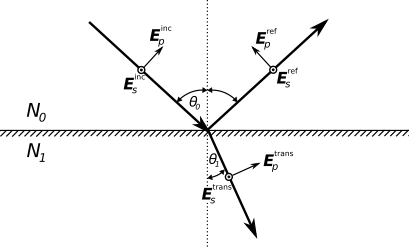
\includegraphics[scale=0.8]{figures/Ch2/SE.png}
    \caption{Light propagating in a medium with refractive index $N_0$ is partially reflected and transmitted when encountering a material with different index $N_1$. The transmitted wave is refracted at an angle $\theta_1$, different from incident angle $\theta_0$, unlike the reflected angle. The polarization state of each wave is defined by the 
    amount of electric field which is p-polarized (parallel to page) and s-polarized (out of page), i.e. in-plane and perpendicular to the plane of incidence, respectively.}
    \label{fig:SE}
\end{figure}
The basic quantity measured with an ellipsometer is the ratio 
\begin{equation}
    \rho = \chi_r/\chi_i,
    \label{eq:ellipsometry_ratio}
\end{equation}
where $\chi_r$ and $\chi_i$ are the complex-number representation of the polarization states of the reflected and incident beams, respectively. Each polarization state is described by the ratio of complex-valued electric fields in the orthogonal p- and s-directions $\chi = E_p/E_s$. As the complex reflection coefficients are defined by the complex reflected and incident electric fields, $r_{pp}=E_{pr}/E_{pi}$ and $r_{ss}=E_{sr}/E_{si}$, we can rewrite equation (\ref{eq:ellipsometry_ratio}) to be
\begin{equation}
    \rho = \frac{r_{pp}}{r_{ss}} = \tan\Psi e^{i\Delta}.
    \label{eq:standard_ellipsometry}
\end{equation}
The so-called ellipsometric angles $\Psi$ and $\Delta$ are the experimentally determined parameters in standard ellipsometry. The angle $\Psi$ describes the relative change in amplitude, while $\Delta$ describes the phase shift.
 
\subsubsection{Generalized ellipsometry}
In the case of an anisotropic sample one must generally include polarization coupling, i.e. the off-diagonal reflection Jones matrix elements $r_{sp}$ and $r_{ps}$ will be non-zero. Because of this, generalized ellipsometry requires at least three values of $\rho$ measured at different polarization states $\chi_i$ which results in three pairs of $(\Psi, \Delta)$. The three complex-valued generalized ellipsometer parameters are defined as
\begin{subequations}
\begin{align}
    \rho_{pp} &= \frac{r_{pp}}{r_{ss}} = \tan \Psi_{pp} e^{i\Delta_{pp}} \\
    \rho_{ps} &= \frac{r_{ps}}{r_{pp}} = \tan \Psi_{ps} e^{i\Delta_{ps}} \\
    \rho_{sp} &= \frac{r_{sp}}{r_{ss}} = \tan \Psi_{sp} e^{i\Delta_{sp}}.
\end{align}
    \label{eq:generalized_ellipsometer_angles}
\end{subequations}

If assuming a sharp interface between the two media, as in figure \ref{fig:SE}, one may combine equation (\ref{eq:standard_ellipsometry}) with equations (\ref{eq:Fresnel_refl_coeff}) and Snell's law while applying $N^2=\epsilon$ to derive a relation connecting the dielectric functions of the two media,
\begin{equation}
    \langle\epsilon\rangle_{pp} =  \sin^2\theta_0\left[ \epsilon_0 + \frac{(1-\rho_{pp})^2}{(1+\rho_{pp})^2}\tan^2\theta_0 \right],
    \label{eq:generalized_pseudo_dielectricfunction}
\end{equation}
known as the \emph{generalized pseudo-dielectric function}\cite{hans_arwin_reviewarticle}. If surface layers can be neglected then $\langle\epsilon\rangle_{pp}=\epsilon_1$. Note that $\epsilon_0$ is the dielectric function of the upper (ambient) media, not the vacuum permittivity. %The pseudodielectric function only works for the case where there is no thin film or overlayer on the surface. If light is able to penetrate the film and reflect from the film/substrate interface the effects of multiple reflections in the film must be accounted for.

\subsubsection{Mueller-matrix ellipsometry}
\label{sec:MM_ellipsometry}
So far we have assumed no depolarization in the sample. When depolarization occurs Jones formalism is no longer valid and one should use Mueller-matrix formalism in describing how an electromagnetic wave interacts with the elements within an ellipsometer (including the sample). Depolarization may be caused by effects such as thickness non-uniformity, non-coherent reflection and backside reflections from a transparent substrate. Furthermore, information such as s- and p-reflectance, and the isotropic and anisotropic ellipsometry parameters may be extracted from the Mueller matrix. In transmission mode, the MM may be useful to observe effects of s- and p-transmittance, optical rotation and circular dichroism\footnote{Dichroism is either when light splits up into distinct beams of different wavelengths, or when light rays experience a different absorption coefficient (diattenuation) depending on its polarization state. Circular dichroism is dichroism involving circularly polarized light, i.e. the differential absorption of left- and right-handed light.}.

The reflection MM of a non-depolarizing sample is readily available from equation (\ref{eq:JonesToMueller}). An isotropic sample is fully described by $\rho = \tan\Psi e^{i\Delta} = r_{pp}/r_{ss}$ as there is no cross-polarization, $r_{sp} = r_{ps} = 0$. It is then fairly straight forward to show that the MM in equation (\ref{eq:JonesToMueller}) becomes block-diagonal as it reduces to
\begin{equation}
    \mathbf{M} = \frac{\abs{r_{pp}}^2+\abs{r_{ss}}^2}{2}
    \begin{pmatrix}
    1 & -N & 0 & 0 \\
    -N & 1 & 0 & 0 \\
    0 & 0 & C & S \\
    0 & 0 & -S & C 
    \end{pmatrix}
    \label{eq:isotropicMM}
\end{equation}
where $N$, $C$ and $S$ are introduced as 
\begin{subequations}
\begin{align}
    N &= \cos 2\Psi                 \\
    C &= \sin 2\Psi \cos \Delta     \\
    S &= \sin 2\Psi \sin \Delta.
\end{align}
    \label{eq:NCS}
\end{subequations}
If the sample in addition is non-depolarizing, these parameters are related as 
\begin{equation}
    N^2+C^2+S^2=1.
    \label{eq:sumNCSsquared=1}
\end{equation}
Furthermore, the complex reflectance ratio can be expressed as \cite{hans_arwin}
\begin{equation}
    \rho = \frac{C+iS}{1+N}.
\end{equation}
In the Mueller matrix approach, an isotropic sample is thus described by three parameters $N$, $C$ and $S$, which reduces to two independent parameters if the sample is non-depolarizing.

Because the MM fully describes the polarization change due to a sample, it has been proved that the additional (in principle redundant) information provided greatly reduces the correlations observed between measured parameters compared to using standard spectroscopic ellipsometry. Examples of benefits gained by Mueller matrix formalism are found when characterizing gratings and anisotropic samples\cite{DeMartino_MMgratingscharacterization}.

%%%%%%%%%%%%%%%%%%%%%%%%%%%%%%%%%%%%%%%%%%%%%%%%
 
\section{Interaction between matter and light}
The interaction between metals and EM waves can be firmly understood by classical electrodynamics, and even metallic nanostructures of a few nanometers in size may be described in the classical sense without resorting to quantum mechanics\cite{maier}. From everyday experience we are well aware of the highly reflective and non-transmittive nature of metals for frequencies up to the visible spectrum. For the lower-frequency regime of microwave and far-infrared (\ac{ir}) radiation
one can in most cases assume the approximation that the metal is a perfect conductor to be valid, due to only a negligible part of the incident radiation actually penetrates into the metal. In the near-IR and visible regime the field penetration is more prominent and leads to increased dissipation. At ultraviolet (\ac{uv}) frequencies metals become dielectric in character and allow for electromagnetic propagation. The attenuation of transmission will however depend on the electronic band structure of the individual metal. Alkali metals exhibit an ultraviolet transparency, while noble metals such as gold and silver experience strong absorption in this regime due to transitions between electronic bands.

In describing these interactions we first begin with Maxwell's equations (\ac{me}) of macroscopic electromagnetism in time domain\cite{griffiths},
\begin{subequations}
\begin{align}
    \nabla \cdot \mathbf{D} &= \rho_{ext}    \\
    \nabla \cdot \mathbf{B} &= 0            \\
    \nabla \times \mathbf{E} &= -\frac{\partial \mathbf{B}}{\partial t}                 \\
    \nabla \times \mathbf{H} &= \frac{\partial \mathbf{D}}{\partial t} + \mathbf{J}_{ext},
\end{align}
\label{eq:ME}
\end{subequations}
which links the four macroscopic fields, the dielectric displacement $\mathbf{D}$, the electric field $\mathbf{E}$, the magnetic field $\mathbf{H}$, and the magnetic induction $\mathbf{B}$, with the external charge and current densities $\rho_{ext}$ and $\mathbf{J}_{ext}$. Furthermore, for linear media, the electric displacement field $\mathbf{D}$ is related to polarization $\mathbf{P}$, which describes the dipole moment per unit volume in the material, as \cite{hans_arwin}
\begin{equation}
    \mathbf{D} = \epsilon_0 \mathbf{E} + \mathbf{P}
    \label{eq:DEP}
\end{equation}
with the constitutive relation in frequency domain
\begin{equation}
   \mathbf{D} = \epsilon_0 \epsilon \mathbf{E}.    
    \label{eq:constitutive relation}
\end{equation}
Here, $\epsilon_0$ is the permittivity of vacuum while $\epsilon$ is the relative permittivity of the medium, which is an intrinsic property of the given material describing the frequency-dependent relation between an applied electric field and the induced displacement field. It is also known as the dielectric function, as it will be called in this thesis. The dielectric function is in general complex for metals and other absorbing materials,
\begin{equation}
    \epsilon = \epsilon_r + i\epsilon_i
\end{equation}
and its relation to the complex refractive index is $N=\sqrt{\epsilon}$.

\subsection{The dielectric function of the free electron gas}

The optical response of metals can be, over a wide frequency range, be explained by a free electron model. That is, a gas of electrons moving against a static background of positive ions. The equation of motion for an electron in the plasma sea under the effect of an external electric field $\mathbf{E}$ can be written as 
\begin{equation}
    m\mathbf{\ddot{x}} + m\gamma\mathbf{\dot{x}} = -e\mathbf{E}
    \label{eq:drude eom}
\end{equation}
with $m$ being the effective optical mass of the electron and $e$ the electron charge. The electron will oscillate in response to the applied field and its motion is damped through collisions described by the characteristic collision frequency $\gamma$. Assuming the driving field has a harmonic time dependence, $\mathbf{E}(t) = \mathbf{E}_0e^{-i\omega t}$, equation (\ref{eq:drude eom}) has a solution describing the electron oscillating as $\mathbf{x}(t)=\mathbf{x}_0e^{-i\omega t}$. The complex amplitude $\mathbf{x}_0$ includes any phase shifts between the driving field and response, and is given by \cite{maier}
\begin{equation}
    \mathbf{x}(\omega) = \frac{e}{m(\omega^2 + i\gamma\omega)} \mathbf{E}(\omega),
    \label{eq:drude x}
\end{equation}
where a Fourier transform has been performed. This displacement from its equilibrium due to the applied electric field results in a polarization $\mathbf{P} = -ne\mathbf{x}$, where $n$ is the electron number density. Inserting this into equation (\ref{eq:drude x}) gives us
\begin{equation}
    \mathbf{P}(\omega) = -\frac{ne^2}{m(\omega^2 + i\gamma\omega)} \mathbf{E}(\omega).
    \label{eq:polarization}
\end{equation}
From the relation (\ref{eq:DEP}) we see that
\begin{equation}
    \mathbf{D}(\omega) = \epsilon_0(1 - \frac{\omega_p^2}{\omega^2 + i\gamma \omega}) \mathbf{E}(\omega)
\end{equation}
where $\omega_p^2 = ne^2/m\epsilon_0$ is the frequency of the collective oscillation of the valence electrons in the metal called the \emph{plasma frequency}, defined as the frequency where the real part of $\epsilon$ is zero\cite{web:dresselhaus}. Finally, from the constitutive relation (\ref{eq:constitutive relation}) we arrive at the dielectric function
\begin{equation}
    \epsilon(\omega) = 1-\frac{\omega_p^2}{\omega^2 + i\gamma \omega}.
    \label{eq:drude response}
\end{equation}
The free electron gas is also known as the Drude model, and thus its dielectric function (\ref{eq:drude response}) is often called the \emph{Drude response} of such a metal.

For noble metals this approach is limited to frequencies below the visual range where interband transitions occur. For such metals an extension is needed in the region $\omega > \omega_p$, where free s-electrons dominates the response while the filled d-band near the Fermi surface causes a highly polarized environment. This residual polarization caused by the positive ion background can be described by adding a term $\mathbf{P_\infty}=\epsilon_0(\epsilon_\infty - 1)\mathbf{E}$ to equation (\ref{eq:DEP}) so that $\mathbf{P}$ in equation (\ref{eq:polarization}) now represents polarization due to free-electron displacement\cite{maier}. This effect is described by $\epsilon_\infty$ and we can rewrite the dielectric function to be
\begin{equation}
    \epsilon(\omega) = \epsilon_\infty-\frac{\omega_p^2}{\omega^2 + i\gamma \omega}.
    \label{eq:drude response2}
\end{equation}

Figure \ref{fig:DrudeGold} illustrates the validity of the free-electron model in the case of gold. Clearly, the model breaks down at visible frequencies and higher as $\epsilon_2$ increases due to interband transitions. 

\begin{figure}
    \centering
    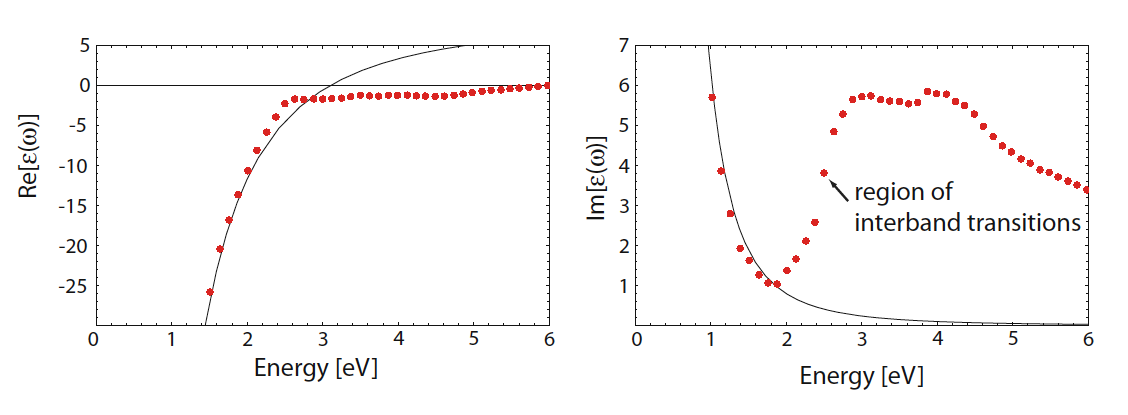
\includegraphics[scale=0.3]{figures/Ch2/DrudeGold.png}
    \caption{The dielectric function $\epsilon(\omega)$ of the free-electron model (solid line) is plotted against experimental values for gold (dots) found in \cite{Johnson&Christy}. Validity of the Drude model breaks down for higher energies due to interband transitions. Figure taken from \cite{maier}.}
    \label{fig:DrudeGold}
\end{figure}

\subsubsection*{Lorentz oscillators}
A method of overcoming these problems at higher frequencies is to add an oscillator term to the equation of motion (\ref{eq:drude eom})
\begin{equation}
    m\mathbf{\ddot{x}} + m\gamma\mathbf{\dot{x}} + m\omega_0^2\mathbf{x} = -e\mathbf{E}
    \label{eq:lorentz eom}
\end{equation}
so that interband transitions are represented by the classical picture of a bound electron with resonance frequency $\omega_0$. The dielectric function can be found by the same procedure as before, solving the equation of motion (\ref{eq:lorentz eom}) and combining equations (\ref{eq:polarization}) and (\ref{eq:constitutive relation}), resulting in
\begin{equation}
    \epsilon(\omega) = 1 - \frac{\omega_p^2}{\omega^2-\omega_0^2+i\omega\gamma}.
    \label{eq:lorentz osc single}
\end{equation}
The plot in figure \ref{fig:lorentzian} shows the typical behaviour of a Lorentz oscillator. [kort forklaring]

This simple model neglects several types of forces\text{\color{red}[??]}; one can more accurately describe the material as a sum of several Lorentz oscillators, generalizing equation (\ref{eq:lorentz osc single}) as
\begin{equation}
    \epsilon(\omega) = \epsilon_\infty - \omega_p^2\sum_{j}\frac{f_j}{\omega^2-\omega_j^2+i\omega\gamma_j}
    \label{eq:lorentz osc sum}
\end{equation}
where $f_j$ is the oscillator strength with $\sum f_j = 1$. Again, it is convenient to summarize all higher energy frequencies into the real-valued parameter $\epsilon_\infty$, describing the relative permittivity at infinite energy, often equating to unity. The Lorentz model is valid only for energies (significantly) lower than the band gap energy \text{\color{red}FINN REF}.
\begin{figure}
    \centering
    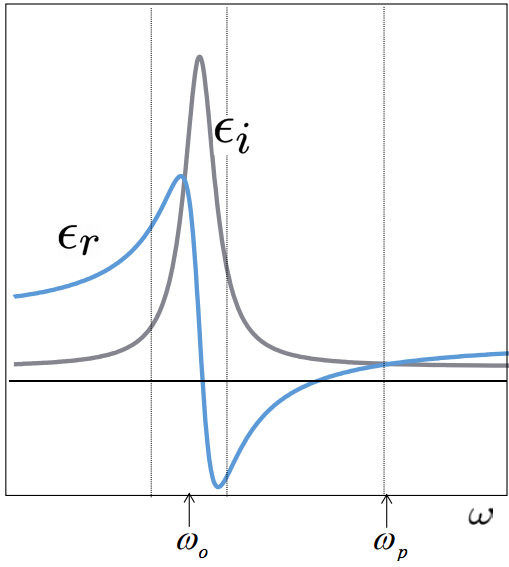
\includegraphics[scale=0.3]{figures/Ch2/Lorentzian.png}
    
    \caption{Typical behaviour of a Lorentz oscillator. Dispersion of light interacting with the material occurs when real part $\epsilon_r$ is non-constant. Absorption occurs when the imaginary part is non-zero, $\epsilon_i \neq 0$. A resonance is centered around $\omega_0$ with half-bandwidth $\gamma$. Figure taken from \cite{web:lorentzMIT}.}
    %https://ocw.mit.edu/courses/electrical-engineering-and-computer-science/6-007-electromagnetic-energy-from-motors-to-lasers-spring-2011/readings/MIT6_007S11_lorentz.pdf
    \label{fig:lorentzian}
\end{figure}


\subsection{Dielectric function of solids over a wide frequency range}
The optical response function has a few general properties that are caused by causality, i.e. its reaction is only dependent on past events and not future events. This leads to the Kramers Kronig relations\cite{hans_arwin}. The Kramer Kronig relations are bidirectional mathematical relations that connects real and imaginary parts of complex functions that are analytic in the upper half-plane, thus applicable to response functions of linear systems where the relationship between input and output is causal\cite{mathmethodsforphysicists}. A consequence of Kramers Kronig relations is that if one of the functions (real part $\epsilon_1$ or imaginary $\epsilon_2$) are determined for all frequencies, then the other part can be calculated for all frequencies as well.

Consider equation (\ref{eq:DEP}), which solved for  $\mathbf{P}$ is
\begin{equation}
    \mathbf{P} = (\epsilon-1)\epsilon_0 \mathbf{E}.
\end{equation}
It is clear that the term $(\epsilon-1)$ represents the optical response as it relates the electric field $\mathbf{E}$ to the polarization $\mathbf{P}$, i.e. the term gives the relation between the \emph{cause} $\mathbf{E}$ and \emph{effect} $\mathbf{P}$. With basis in equation (\ref{eq:DEP}) and taking into account causality, that $\mathbf{E}$ must precede a response $\mathbf{P}$ implying that $\mathbf{P}$ should vanish for $t<0$, as well as Cauchy's residue theorem for complex functions, it can be shown that the Kramer Kronig integrals are \cite{web:dresselhaus}\cite{hans_arwin}
\begin{subequations}
    \begin{align}
        \epsilon_1 - 1 = \frac{2}{\pi}\mathscr{P}\int_0^\infty\frac{\epsilon_2(\omega')\omega'}{\omega'^2-\omega^2}d\omega'    \\
        \epsilon_2 = -\frac{2\omega}{\pi}\mathscr{P}\int_0^\infty\frac{\epsilon_1(\omega')-1}{\omega'^2-\omega^2}d\omega'
    \end{align}
    \label{eq:KramerKronig}
\end{subequations}
where $\mathscr{P}$ denotes the principal part of the integral.

Both dispersion (described by $\epsilon_1$) and absorption (described by $\epsilon_2$) originate from the same underlying process, excitation of dipoles in the material. If the dipoles can follow the field instantaneously in a frequency region, there will be no absorption ($\epsilon_2 = 0$). For the same reason there will be no dispersion, as $\epsilon_1$ is constant. In the frequency region around a relaxation (see figure \ref{fig:lorentzian}), the dipoles will still try to match the field but cannot follow it completely. The dipoles will not move as much as at lower frequencies and thus the polarization becomes smaller ($\epsilon_1$ decreases). At the same time absorption occurs ($\epsilon_2 \neq 0$) because energy is tapped from the electromagnetic field into the dipoles and then subsequently into the material. No dispersion can occur if there is no absorption and vice versa. This is the physical interpretation of the Kramer-Kronig relations, that absorption and dispersion are coupled properties of the same phenomenon\cite{hans_arwin}. 

\begin{figure}
    \centering 
    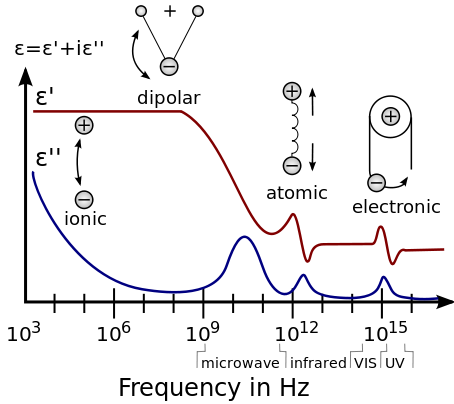
\includegraphics[scale=0.5]{figures/Ch2/DielectricResponses.png}
    \caption{Frequency variation of the dielectric function, showing various dielectric mechanisms: ionic and dipolar relaxation, and resonances of vibrational and electric oscillators. Figure from \cite{wiki_dielectricfunction}.}
    \label{fig:dielectricresponses}
    % https://en.wikipedia.org/wiki/Permittivity#cite_note-5
\end{figure}

Figure \ref{fig:dielectricresponses} shows a dielectric function over a wide frequency range. One quickly observes that at each relaxation frequency of $\epsilon_1$ there is an associative peak in absorption $\epsilon_2$. Starting at $\omega=0$, the dielectric function is composed of contributions from each polarization mechanism (permanent dipoles, vibrational oscillators and electronic oscillators), with the lowest-frequency mechanism contributing the most. As the frequency increases, the permanent dipoles cannot respond and the real part $\epsilon_1$ drops to a value at a frequency low compared to the characteristic vibrational frequency. As the frequency increases through the vibrational region, $\epsilon_1$ oscillates and settles down at a low-frequency limit for electronic modes. For frequencies far above all absorption bands $\epsilon_1$ approaches the free-space value 1; the frequencies are so high that none of the polarization mechanisms can respond, see equation (\ref{eq:KramerKronig})\cite{BH}.
%\begin{itemize}
    %\item [Dispersion occurs when real part $\epsilon_1$ is non-constant. Absorption occurs when the imaginary part is non-zero, $\epsilon_2 \neq 0$.]
    
    %\item Studying the dielectric function as a function of frequency over a vast spectrum, one observes that energy is mainly absorbed at relaxation or resonance frequencies. Why does it not cost energy to excite dipoles at lower frequencies? It does in fact cost energy, but this energy is paid back to the field from the dipoles. This is called virtual dispersion.
    
    %\item For frequencies far above all absorption bands $\epsilon_1$ approaches the free-space value 1; the frequencies are so high that none of the polarization mechanisms can respond.
    
   % At $\omega=0$, the dielectric function is composed of contributions from permanent dipoles, vibrational oscillators and electronic oscillators. As the frequency increases, the permanent dipoles cannot respond and the real part $\epsilon_1$ drops to a value at a frequency low compared to the characteristic vibrational frequency. As the frequency increases through the vibrational region, $\epsilon_1$ oscillates and settles down at a low-frequency limit for electronic modes. After finally the frequency reaches beyond the point where all electronic modes are exhausted, $\epsilon_1$ approaches 1.
    
  %  At each relaxation frequency of $\epsilon_1$ there is an associative peak in absorption $\epsilon_2$.
 %   \item "For noble metals such as gold or silver on the other hand, transitions between electronic bands lead to strong absorption in this regime." -Maier
%\end{itemize}


\subsection{Joule heating}
Energy of the light incident on a material can be dissipated into heat. Resistive (or ohmic) heating is a process by which an electric current passing through a conductor produces heat. In microscopic terms, resistive heating is caused by interactions between the moving particles of the electron plasma and the atomic ions of the material. The electrons are accelerated by an electric field causing them to collide with the ions, resulting in random scattered motion. These thermal fluctuations increases the temperature of the system. Resistive heating defined as power input per unit volume due to electric current is \cite{jackson}
\begin{equation}
    \frac{dP_{\text{resistive}}}{dV} = \mathbf{J}\cdot\mathbf{E}.
    \label{eq:Resistive_heating_dP/dV}
\end{equation}
Here, $\mathbf{J}$ is the current density defined from the constitutive relation $\mathbf{J}=\sigma\mathbf{E}+\mathbf{J}_{ext}$, where $\sigma$ is the conductivity of the electron plasma.  Solving equation (\ref{eq:Resistive_heating_dP/dV}) with respect to $P_{\text{resistive}}$ we get
\begin{equation}
    P_{\text{resistive}} = \int_V \mathbf{J}\cdot\mathbf{E} dV,
    \label{eq:Resistive_heating_P}
\end{equation}
which result in heat dissipation in the material of volume $V$.

\subsection{Effective medium approximation}
This section will give a rough introduction to effective medium theory, and specifically the Bruggeman effective medium model. Effective medium approximations (\ac{ema}) refer to analytical modeling that describe the macroscopic properties of composite materials. A heterogeneous material with inhomogeneities of sizes sufficiently smaller than the wavelength of light will appear as a homogeneous material, i.e. there will be no scattering from the material and its optical properties may be summarized by an effective dielectric function $\epsilon_\text{eff}$\cite{hans_arwin}. EMAs are often used to model nanostructured surfaces, metamaterials, surface roughness, or mixed materials. They are convenient when used together with ellipsometric measurements to characterize nanostructures of a sample.

\begin{figure}
\begin{subfigure}{0.5\textwidth}

    \begin{subfigure}{\textwidth}
        \flushright
        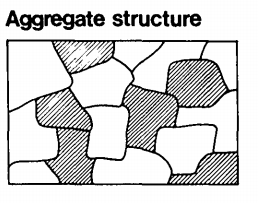
\includegraphics[width=0.7\linewidth]{figures/Ch2/EMA2.png}
    \end{subfigure}
   
    \begin{subfigure}{\textwidth}
        \flushright 
        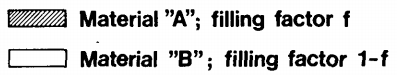
\includegraphics[width=0.7\linewidth]{figures/Ch2/EMA3.png}
    \end{subfigure}
%
\end{subfigure}
\begin{subfigure}{0.5\textwidth}
    \flushleft
    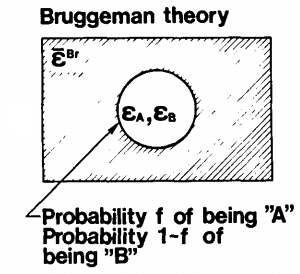
\includegraphics[width=0.7\linewidth]{figures/Ch2/EMA1.png}
%
\end{subfigure}
\caption{(left) An aggregate structure, where two materials are mixed on a random basis, (right) the corresponding random unit cell used to derive the effective dielectric function for the Bruggeman theory. Figure from \cite{Niklasson_EMAmodels}.}
\label{fig:EMA_bruggeman}
\end{figure}

An effective medium model assumes that the macroscopic optical response of a microstructure of heterogeneous multi-phase media may be estimated by a random unit cell (an effective medium) that should not be detectable in an experiment using EM radiation confined to a specified wavelength range. Put differently, the extinction of the random unit cell should be the same as if it were replaced with a material with the effective dielectric function. The Bruggeman effective medium model assumes the material has an aggregate structure as shown in figure \ref{fig:EMA_bruggeman}, which demands a random unit cell which guarantees the structural equivalence of the two constituents. The cell is therefore a sphere whose dielectric function is $\epsilon_A$ with probability $f_A$, and $\epsilon_B$ with probability $f_B$. The Bruggeman effective medium expression is known as
\begin{equation}
    0 = f_A \frac{\epsilon_A - \epsilon_\text{eff}}{\epsilon_A+2\epsilon_\text{eff}} + f_B \frac{\epsilon_B - \epsilon_\text{eff}}{\epsilon_B+2\epsilon_\text{eff}}
    \label{eq:EMA_Bruggeman}
\end{equation}
where $f_A$ is the volume fraction of material $A$ and $f_B = 1 - f_A$ is the volume fraction of material $B$\cite{hans_arwin}.
\section{Plasmonics}
The field of plasmonics explores how electromagnetic fields may be confined and/or enhanced over sub-wavelength dimensions. It is based on the interaction between light and the conduction electrons at a metallic interface or metallic nanoparticles, resulting in an enhanced electromagnetic field over dimensions smaller than the wavelength of light. There are two types of surface plasmons. One is a dispersive electromagnetic wave coupled to the electron plasma of a conducting material propagating along the interface between the conductor and a dielectric. This is called a surface plasmon polariton resonance (\ac{sppr}), or just SPP or \ac{spr}. The other type is a non-propagating excitation of the electron plasma of metallic nanostructures coupled to an incident electromagnetic field called a localized surface plasmon resonance (\ac{lspr}). This thesis will focus on describing the latter.

\subsection{Localized surface plasmons}
LSPRs occur naturally in the scattering of an oscillating electromagnetic field from a small, sub-wavelength conductive nanoparticle. The surface curvature of the particle acts as an effective restoring force on the driven electron-plasma so that a resonance arises, field amplifications both inside and in the near-field zone outside the particle. The spectral location of the LSPR is characteristic for the size, the shape, the material and the surrounding medium of the nanoparticle.

\subsubsection{Normal modes}
The interaction process between light and a sub-wavelength metal particle with diameter $d$ may be examined by using the \emph{quasi-static approximation}, assuming $d\ll \lambda$. The  phase  of  the  harmonically  oscillating  field is then considered to be practically constant over the particle volume, i.e. the particle is assumed to be surrounded by an electrostatic field. By ignoring spatial retardation effects over the particle the spatial field distribution can be calculated, while the harmonic time dependence may be added to the solution afterwards. This approximation has been shown to be reasonable for spherical and ellipsoidal particles with dimensions below 100 nm when illuminated by visual or near-IR light\cite{maier}.

\begin{figure}
    \centering
    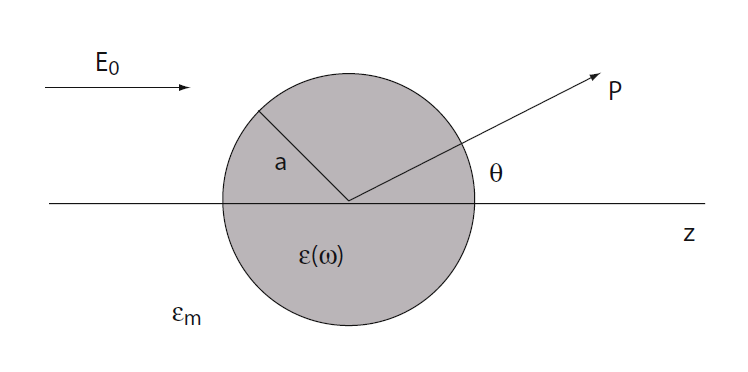
\includegraphics[scale=0.6]{figures/Ch2/SphereNormalMode.PNG}
    \caption{A metallic sphere with radius $a$ and dielectric function $\epsilon(\omega)$ placed in an ambient medium with dielectric constant $\epsilon_m$. The particle is subject to an external electrostatic field $E_0$. Figure taken from \cite{maier}.} 
    \label{fig:normalmode}
\end{figure}

We will from here on concider the example of a homogeneous, isotropic sphere of radius $a$ located at the origin in a uniform, static electric field $\mathbf{E}=E_0\mathbf{\hat{z}}$. The surrounding isotropic non-absorbing medium has dielectric constant $\epsilon_m$ while the dielectric response of the sphere is $\epsilon(\omega)$. See figure \ref{fig:normalmode}. The distribution of the electric field $\mathbf{E}=-\nabla \Phi$ can then be calculated from the solution of the Laplace equation $\nabla ^2 \Phi = 0$\cite{griffiths}. Since the problem has azimuthal symmetry, the general solution is\cite{jackson}
\begin{equation}
    \Phi (r,\theta) = \sum_{l=0}^\infty[A_lr^l + B_lr^{-(l+1)}] P_l(\cos\theta),
\end{equation}
with Legendre polynomials $P_l(\cos\theta)$ of order $l$, and $\theta$ being the angle between z-axis and the position vector $\mathbf{r}$. The potentials must be finite at the origin, the solution for the potentials inside and outside the sphere may therefore be written as
\begin{subequations}
\begin{align}
    \Phi_{in}(r,\theta) &= \sum_{l=0}^\infty A_l r^l P_l(\cos\theta) \\
    \Phi_{out}(r,\theta) &= \sum_{l=0}^\infty [B_l r^l + C_l r^{-(l+1)}] P_l(\cos\theta). 
\end{align}
\end{subequations}
The coefficients $A_l$, $B_l$, $C_l$ may be determined from the boundary conditions at $r \to \infty$ and $r=a$. On the former limit it is required that $\Phi_{out} \to -E_0z = -E_0r\cos\theta$ which requires $B_1 = -E_0$ and $B_l=0$ for $l\neq1$. The remaining coefficients are found from the latter limit on the particle surface, by equating tangential components of the electric field outside and inside the sphere at $r=a$, and similarly by equating the normal components of the displacement field. This leads to $A_l = C_l = 0$ for $l \neq 1$, and by calculating the remaining $A_1$ and $C_1$ the potentials end up as\cite{jackson}    
\begin{subequations}
\begin{align}
    \Phi_{in} &= -\frac{3\epsilon_m}{\epsilon+2\epsilon_m}E_0 r \cos\theta  \\
    \Phi_{out} &= -E_0 r \cos\theta + \frac{\epsilon-\epsilon_m}{\epsilon+2\epsilon_m} E_0 a^3 \frac{\cos\theta}{r^2}.
    \label{eq:test}
\end{align}  
\end{subequations}
The last equation (\ref{eq:test}) may be interpreted physically as $\Phi_{out}$ describing the superposition of the applied field and that of a dipole located at the particle center. It is therefore interesting to rewrite $\Phi_{out}$ in terms of dipole moment $\mathbf{p}$ as
\begin{subequations}
\begin{align}
        \Phi_{out} &= -E_0 r \cos\theta + \frac{\mathbf{p}\cdot \mathbf{r}}{4\pi\epsilon_0\epsilon_mr^3}    \\
        \mathbf{p} &= 4\pi\epsilon_0\epsilon_m a^3 \frac{\epsilon-\epsilon_m}{\epsilon+2\epsilon_m} \mathbf{E_0}.
    \end{align}
    \label{eq:LSPR_dipolemoment}
\end{subequations}
Thus, the applied field induces a dipole moment inside the sphere proportional to the electric field. The radiation of this dipole leads to \emph{scattering} of the plane wave by the sphere, which can be represented as radiation by a point dipole as here. Introducing polarizability $\alpha$, defined as $\mathbf{p}=\epsilon_0\epsilon_m\alpha\mathbf{E}_0$, results in \footnote{For a particle in air, i.e. $\epsilon_m=1$, equation (\ref{eq:polarizability}) is more famously known as the Clausius-Mossotti relation when the particle is a sphere.}
\begin{equation}
    \alpha = 4\pi a^3 \frac{\epsilon-\epsilon_m}{\epsilon+2\epsilon_m}.
    \label{eq:polarizability}
\end{equation}
Polarizability describes a material's ability to form instantaneous dipoles, or in other words, the relative tendency of a charge distribution to have its charges displaced by an external electric field. We see from (\ref{eq:polarizability}) that the polarizability is proportional to the particle radius cubed, and it is apparent that a resonant behaviour occurs when $|\epsilon+2\epsilon_m|$ is at a minimum. In the case of a small or slowly varying $\text{Im}[\epsilon]$ this resonance condition simplifies to 
\begin{equation}
    \text{Re}[\epsilon(\omega)] = -2\epsilon_m.
    \label{eq:frolich}
\end{equation}
This is known as the Frölich condition, and the associated mode is called the \emph{dipole surface plasmon} of the metal nanoparticle\cite{maier}.

From equation (\ref{eq:frolich}) it is evident that the resonance frequency depends strongly on the dielectric environment: for a Drude metal with a small Im$[\epsilon(\omega)]$ the resonance red-shifts as the dielectric constant of the surroundings $\epsilon_m$ increases. Metal nanoparticles are therefore a very promising mean of optical sensing of changes in refractive index.

A consequence of a resonantly enhanced polarizability is an accompanying enhancement in the metal nanoparticle's ability to scatter and absorb light. From a Mie theory approach for particles small compared with wavelength one can find the cross sections for scattering and absorption\cite{BH},
\begin{subequations}
    \label{eq:cross_sections}
    \begin{align}
        C_{sca} &= \frac{k^4}{6\pi}|\alpha|^2 = \frac{8\pi}{3} k^3 a^6 \abs{ \frac{\epsilon-\epsilon_m}{\epsilon+2\epsilon_m} }^2 \\
        C_{abs} &= k\text{Im}[\alpha] = 4 \pi k a^3 \text{Im}\left[ \frac{\epsilon-\epsilon_m}{\epsilon+2\epsilon_m} \right]
    \end{align}
    \label{eq:CrossSections}
\end{subequations}
with $k=2\pi/\lambda$. Equations (\ref{eq:CrossSections}) are valid for all spherical particles $a\ll\lambda$ with different material properties from its ambient, no metallic assumption is made in the derivation, and the equations are therefore also valid for dielectric scatterers. Due to the rapid scaling of $C_{sca} \propto a^6$ it is very difficult to pick out small objects from a background of large scatterers. Equations (\ref{eq:cross_sections}) also show that for metallic nanoparticles both absorption and scattering (and thus extinction) is resonant at the dipole particle plasmon resonance when the Frölich condition is met. 

\subsection{Particle size and shape effects}
%Equation (\ref{eq:polarization}) suggests that particle size has no effect on spectral position and width of the plasmon resonance. There are indeed [such effects/links], however, but they are not captured by the quasi-static approximation. 
Two regimes can be considered when investigating how particle size affects the LSPR: larger particles where retardation effects are non-neglible, and very small metal particles with dimensions smaller than the mean free path of its oscillating electrons. The latter regime regards particles of radius $a<10$ nm\cite{maier}, as this thesis does not consider particles of such size we will focus our efforts on the former.

For particles with larger dimensions the quasi-static approximation is no longer valid as there will be significant phase-changes of the driving field over the particle volume. A rigorous electrodynamic Mie theory approach is needed to find the polarizability for such a spherical particle, the interested reader can find the equation and derivation in\cite{Kuwata2003}\cite{LargeParticlesLSPR_maier}. For such particles there is found to be an energy shift of the plasmon resonance due to the retardation of the depolarization field\footnote{In the case that the polarization of the dipoles is induced by an external field, the polarization field $\mathbf{P}$ opposes the applied field $\mathbf{E}$ and is sometimes called a depolarization field.} inside the particle\cite{LargeParticlesLSPR_maier}. Figure \ref{fig:LSPR_largeParticles} shows the change in local field enhancement as particle size of silver spheres is increased. The dipole resonance red-shifts and is strongly broadened along with a drastic decrease in enhancement. The spectral shift of plasmon resonance to longer wavelengths suggests that interband transitions (described by an increase in $\epsilon_2$) have less effect as the resonance moves away from the band gap energy\cite{maier}. %[copyFraMaier:]Intuitively, this can be understood by recognizing that the distance between the charges at opposite interfaces of the particle increases with its size, thus leading to a smaller restoring force and therefore a lowering of the resonance frequency.
As the particle size increases the dipole plasmon resonance is severely damped, mainly due to \emph{radiation damping}\cite{Wokaun_RadiationDamping}. Radiative damping is the direct decay of a surface plasmon (the coherent electron oscillation on the metal surface due to coupling with the external EM wave) into photons\cite{Kokkinakis_RadiativeDecay}.
\begin{figure}
    \centering
    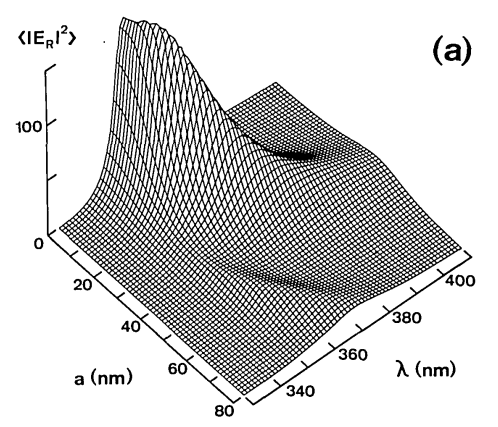
\includegraphics[width=0.5\linewidth]{figures/Ch2/LSPR_on_largeparticles.png}
    \caption{(a) Electric field enhancement on the surface of silver spheres of radius $a$. The radial surface field $E_R$ is normalized by the incident field. Absolute maximum occurs at $a=12.5$nm for $\lambda_{max}=357$nm (electrostatic limit $a=0$nm: $\lambda_{max}=355$nm). LSPR enhancement decreases for larger particles, in addition it is shifted to longer wavelengths and broadened. The surface field is dominated by dipolar contribution. The smaller resonance for $a>40$nm is due to quadrupole contribution. Figure taken from \cite{LargeParticlesLSPR_maier}.}
    \label{fig:LSPR_largeParticles}
\end{figure}

Particle shape effects will be briefly investigated by studying an ellipsoid, being the most general smooth particle, in the electrostatics approximation. Consider an ellipsoid with semiaxes $a>b>c$ with a dipole moment induced by a uniform electrostatic field parallel to one of its principal axes. The dipole moment, and hence the polarizability of the ellipsoid, will vary depending on which of the three axes the applied field is parallel to. Then, for an ellipsoid with dielectric function $\epsilon$ set in an ambient medium $\epsilon_m$, the polarizability is given by \cite{BH}
\begin{equation}
    \alpha_i = \frac{4\pi abc}{3} \frac{\epsilon-\epsilon_m}{\epsilon_m + L_i(\epsilon-\epsilon_m)} \quad\quad i=1,2,3
    \label{eq:polarizability_ellipsoid}
\end{equation}
when the electric field is directed along the $i$th axis of the ellipsoid corresponding to the parameters $a$, $b$ and $c$, respectively. Here, $L_i$ are the geometrical factors related to the shape of the particle, where $\sum_i L_i=1$ and $L_1\leq L_2 \leq L_3$. For a sphere we have $L_1=L_2=L_3=1/3$, and (\ref{eq:polarizability_ellipsoid}) reduces to equation (\ref{eq:polarizability}).

\begin{figure}[h]
    \centering
    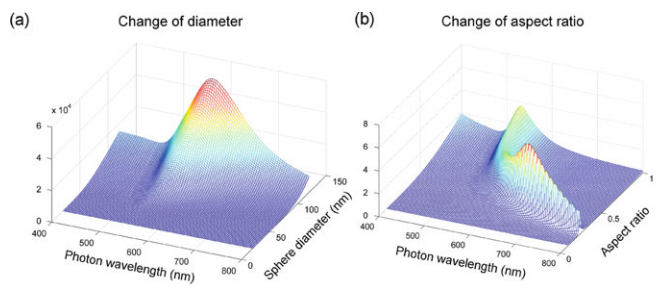
\includegraphics[width=\linewidth]{figures/Ch2/TuningLSPR.png}
    \caption{Scattering cross section plotted against changes in (a) the diameter and (b) the aspect ratio of a gold nanosphere in the spectrum around a surface plasmon polariton resonance. Figure from \cite{Trugler_metallicnanoparticles}.}
    \label{fig:tuning_plasmon_resonance}
\end{figure}

The resonance of the surface plasmon polariton may be tuned by changing the size and shape of a metallic nanoparticle, as shown in figure \ref{fig:tuning_plasmon_resonance}. It is clear that changing the aspect ratio of the particle has greater impact on the resonance position than changing its diameter. The resonance intensity in \ref{fig:tuning_plasmon_resonance}b has a maximum for an aspect ratio between $0.3$ and $0.4$\cite{Trugler_metallicnanoparticles}\cite{Becker_aspectratio_goldnanorods}.

\subsection{Coupling between LSPRs}
Until now we have regarded the LSPR in a single metallic nanoparticle, and the shift in resonance frequency caused by changes in particle shape and size. One may expect additional shifts in frequency when several such particles are brought together, due to electromagnetic interaction between neighbouring localized modes. 

The dipolar approximation may be assumed when the particle sizes are much smaller than the interparticle distance, $a\ll d$, so that the particles may be treated as point dipoles. For closely spaced particles, $d\ll \lambda$, the near-field interactions dominate with a distance dependence of $d^{-3}$ (see equation (\ref{eq:LSPR_dipolemoment})) and the particle ensemble may be described as an array of dipoles interacting with their near-field\cite{maier}. By considering the Coulomb forces associated with the polarization of particles in an array of interacting point dipole particles, one can intuitively see that interparticle coupling will lead to shifts in the LSPR spectral position when compared to an isolated particle. Figure \ref{fig:nearfield_coupling} illustrates how the restoring force, acting on the oscillating electrons in each particle, is either increased or decreased by the charge distribution of their neighbouring particles. The particle's internal dipole moment induced by the applied external field affects its neighbouring particle's induced dipole moment. This leads to a blueshift of the plasmon resonance for transversal polarization of the exciting light, and a redshift for longitudinal polarization.
\begin{figure}
    \centering
    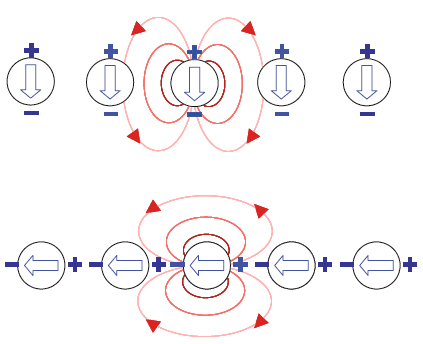
\includegraphics[width=0.5\linewidth]{figures/Ch2/nearfieldcoupling.PNG}
    \caption{Near-field coupling between metallic nanoparticles when light incident from the side is s-polarized (top) and p-polarized (bottom). Thick arrows indicate each particle's internal dipole moment. Figure from \cite{maier}.}
    \label{fig:nearfield_coupling}
\end{figure}

For larger particle seperations the external dipole fields become spherical in shape and the far-field dipolar coupling dominates with a distance dependence of $d^{-1}$\cite{maier}. This coupling via diffraction has been studied for two-dimensional arrays of gold nanoparticles with various lattice constants\cite{Lamprecht_LSPRfarfieldcoupling}. Figure \ref{fig:farfield_coupling} shows that far-field coupling influences the plasmon resonance both in terms of peak strength and spectral width. The spectral shift and broadening of the plasmon resonances are attributed to the periodicity of a square array. The dipolar fields of neighbouring particles are superimposed with their respective phase shifts, which depend on the interparticle distance\cite{Lamprecht_LSPRfarfieldcoupling}.


\begin{figure}
    \centering
    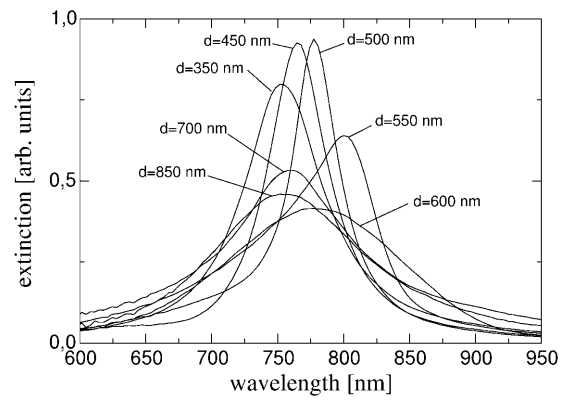
\includegraphics[width=0.5\linewidth]{figures/Ch2/farfieldcoupling.png}
    \caption{Extinction spectra for square two-dimensional gratings of circular gold nanoparticles (height $14$ nm, diameter $150$ nm) on an indium-tin-oxide coated glass substrate with grating constant $d$. Figure from \cite{Lamprecht_LSPRfarfieldcoupling}.}
    \label{fig:farfield_coupling}
\end{figure}

\section{Diffraction anomalies in periodic nanostructures}
Periodic metallic nanostructures are known to show certain intensity anomalies. In 1902 Wood discovered anomalies in his data when studying the spectrum of an optical metallic diffraction grating, remarking that the anomalies were present only for p-polarized light, i.e. when the magnetic field is parallel to the grating grooves\cite{Wood1902}. It was later discoverd by Fano that there could be distinguished two types of such anomalies\cite{fano1941}. The first type is an abrupt change in reflectivity appearing at sharply defined wavelengths at a given angle of incidence of the incoming light, known today as \emph{Rayleigh anomalies}\cite{plasmonics_wood}. These are independent of the metal on which the grating was ruled on, and are furthermore found to also occur (albeit weakly) for incident light with the electric field polarized parallel to the grooves, i.e. s-polarization, if the grooves are sufficiently deep\cite{RayleighWood_simonsen}. The second type is a diffuse anomaly, consisting generally of a minimum and a maximum of intensity, associated with the excitation of a SPP due to both the geometry and the optical properties of the metal grating\cite{RayleighWood_simonsen}\cite{fano1941}. A thorough explanation and derivation of the latter type, known as \emph{Wood anomaly}, can be found in \cite{plasmonics_wood}. Both anomalies are strongly dependent on the grating geometry, the presence of sharp edges in the profile of the grooves being a necessary condition for their existence\cite{fano1941}. This section will focus on explaining the Rayleigh anomalies.

 It was first shown by Rayleigh that these anomalies occur at wavelengths where the diffracted light of a given order disappears at grazing angles along the grating surface\cite{Rayleigh_onWood1907}\cite{Rayleigh_onGratings1907}. For regular periodic structures of nanoparticles on a transparent substrate, a diffracted beam will disappear as it attempts to cross the boundary between the ambient (usually air) and substrate media. The transition between air and substrate is prohibited due to different dispersion relations for light in both media. The diffraction mode is said to be cut off at a Rayleigh cutoff wavelength $\lambda_R$, resulting in a sudden change in reflection. There are two types of Rayleigh cutoff wavelengths for every mode; one for the disappearance of an "air" diffraction mode, where the mode crosses the boundary from air to substrate; the other for the disappearance of a "substrate" diffraction mode, crossing the boundary from substrate to air. %Assuming a square array with lattice constant $a$ and incident light aligned along the array (azimuthal angle $\phi_0=0$), the simplest air and substrate $\lambda_R$ are given by \text{\color{red}CITE}%https://journals.aps.org/prl/pdf/10.1103/PhysRevLett.101.087403
%\begin{equation}
%    \lambda_R^m = \frac{a}{m}[n_i \pm \sin\theta_0]
%\end{equation}
%where $m$ is an integer defining the diffraction mode, and $n_i$ the refractive index of whichever ambient or substrate medium the beam is crossing from. 
When light with wavelength $\lambda_R$ is incident on the array, one of the diffracted waves will travel exactly along the substrate surface and subsequently will interact with other nanoparticles. It is therefore interesting to note that if $\lambda_R$ is close to the wavelength of an individual nanoparticle's LSPR, very sharp plasmon resonances may be obtained as energy from the incident light is transferred into localized plasmon modes in the narrow wavelength range near the Wood anomaly\cite{narrowLSPRfromDiffractionCoupling}.

%For the $n$th diffraction order scattered along the grating surface these anomalies will occur at wavelengths
%\begin{equation}
%\lambda_n = \frac{d}{n}(\pm1-\sin\theta_0),
%\end{equation}
%where $d$ is the grating period, $\theta_0$ the angle of incidence and $n$ the diffraction order integer.

The remaining part of this section will derive an equation that can determine all Rayleigh anomalies, i.e. the condition for a scattered or transmitted wave vector along the surface of a diffraction grating. 

Consider an array of scatterers where the position of each unit cell describing the periodicity is given by the lattice vector
\begin{equation}
    \mathbf{x}^\mathbf{l}=l_1\mathbf{a}_1+l_2\mathbf{a}_2
\end{equation} 
where $\mathbf{a}_{1,2}$ are two noncollinear primitive translation vectors and $\mathbf{l}=(l_1,l_2)$ with $l_{1,2}$ being integers labeling the unit cells. The associated reciprocal lattice is given by
\begin{subequations}
\label{eq:reciprocalLatticeVector}
\begin{align}
    \centering
    \mathbf{G}_\parallel^\mathbf{m} = m_1\mathbf{b}_1 + m_2\mathbf{b}_2 
\end{align}
where $\mathbf{m}=(m_1,m_2)$ are integers, $\mathbf{b}_1$ and $\mathbf{b}_2$ denote the primitive translation vectors of the reciprocal lattice defined by $\mathbf{a}_i\cdot\mathbf{b}_j=2\pi\delta_{ij}, i,j=1,2$ \footnote{Kronecker delta, $\delta_{ij} =
    \begin{cases}
            1, &         \text{if } i=j,\\
            0, &         \text{if } i\neq j.
    \end{cases}$}. 
In terms of polar coordinates the reciprocal lattice vector becomes
\begin{equation}
    \mathbf{G}_\parallel^\mathbf{m} = G_\parallel^\mathbf{m} \langle \cos\phi_\mathbf{m}, \sin\phi_\mathbf{m},0 \rangle
\end{equation} 
where $G_\parallel^\mathbf{m}$ is the length of the reciprocal lattice vector, which for a rectangular lattice ($\mathbf{b}_1\perp\mathbf{b}_2$) is
\begin{equation}
    G_\parallel^\mathbf{m} = 2\pi\sqrt{\frac{m_1^2}{a_1^2} + \frac{m_2^2}{a_2^2}}.
\end{equation}
\end{subequations}
Figure \ref{fig:reciprocallattice} shows a schematic diagram of the reciprocal array in the case of a square lattice, $a_1=a_2=a$. Azimuthal angle of the incident light is defined as the angle $\phi_0$ between the vectors $\mathbf{k}_\parallel$ and  $\mathbf{G}_\parallel^{(10)}$ as shown in the figure, where $\mathbf{k}_\parallel=k\sin\theta_0\langle\cos\phi_0,\sin\phi_0,0\rangle$  is the component of incident wave vector parallel to the substrate surface. Similarly, the angle $\phi_\mathbf{m}$ of reciprocal lattice point $\mathbf{m}$ is the angle between $\mathbf{G}_\parallel^{(10)}$ and $\mathbf{G}_\parallel^\mathbf{m}$.
\begin{figure}
    \centering
    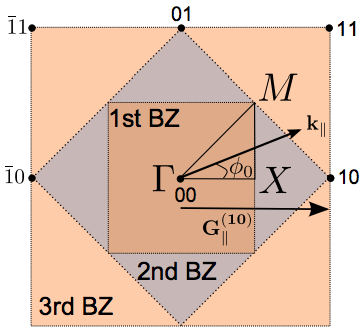
\includegraphics[scale=0.45]{figures/Ch2/ReciprocalLattice.png}
    \caption{Schematic overview of the reciprocal lattice of a square array. Azimuthal angle of incident wave is defined as $\phi_0\angle(\mathbf{G_\parallel^{(10)}},\mathbf{k}_\parallel)$. The boundary of the first three Brillouin zones are indicated by dotted lines, accompanied by critical symmetry points. Figure taken from \cite{Brakstad:15}.}
    \label{fig:reciprocallattice}
\end{figure}

Let us now define the diffraction wave vector into the air or substrate, parallel to the interface, as \cite{KretschmannMaradudin}
\begin{equation}
    \mathbf{q}_\parallel^\mathbf{m} = \mathbf{k}_\parallel + \mathbf{G}_\parallel^\mathbf{m}.
    \label{eq:RayleighDiffractedBeam}
\end{equation}
The dispersion of Rayleigh anomalies in a two-dimensional planar grating follows the relation $\mathbf{q}_\parallel^\mathbf{m} = \mathbf{q}^\mathbf{m}$, which suggests that 
\begin{equation}
    \abs{\mathbf{q}_\parallel^\mathbf{m}}^2 = n_i^2 k^2
    \label{eq:RayleighLineCondition}
\end{equation}
is the condition for a grazing diffracted wave, where $n_i$ is the refractive index of either ambient or substrate, depending on which side of the interface the light is approaching from. By using equations (\ref{eq:reciprocalLatticeVector})-(\ref{eq:RayleighLineCondition}) one may derive an equation determining all Rayleigh anomalies, resulting in \cite{Brakstad:15}
\begin{equation}
    k^2 - \frac{2\sin\theta_0G_\parallel^\mathbf{m}\cos(\phi_m-\phi_0)}{n_i^2-\sin^2\theta_0}k - \frac{(G_\parallel^\mathbf{m})^2}{n_i^2-\sin^2\theta_0} = 0,
    \label{eq:RayleighLines}
\end{equation}
that is, solving equation (\ref{eq:RayleighLines}) with respect to $k=2\pi/\lambda_R$ for a given angle of incidence $(\theta_0,\phi_0)$ tells us which wavelengths of incident light that will result in diffracted modes propagating exactly along the air/substrate interface. 

It is known that for a wave in a periodic medium whose wave vector terminates on the boundary of a Brillouin zone (\ac{bz}), satisfy the condition of diffraction\cite{kittel}. Therefore, for a square lattice, inserting $G_\parallel^{\bar{1}0}$, $G_\parallel^{\bar{1}\bar{1}}$, or $G_\parallel^{\bar{2}0}$ as $G_\parallel^{\mathbf{m}}$ in equation (\ref{eq:RayleighLines}) results in the boundaries of the first, second or third Brillouin zones, respectively, when solved over $\phi_0\in[0^\circ,45^\circ]$ for a fixed polar angle of incidence $\theta_0$ and refractive index $n_i$. The boundaries of the 1st and 2nd BZ of a two-dimensional square lattice are shown in figure \ref{fig:reciprocallattice}.
 %https://books.google.no/books?id=HtjgrALoyAMC&lpg=PR5&ots=pUIcVvIXfY&dq=%22Giessen%22%20Photonic%20Crystals%3A%20Advances%20in%20Design%2C%20Fabrication%2C%20and%20Characterization&lr&hl=no&pg=PA89#v=onepage&q=rayleigh%20anomal&f=false ctrl+f rayleigh anom Chapter 5 H.Giessen et al som igjen refererer til https://journals.aps.org/prb/pdf/10.1103/PhysRevB.58.6779


\subsection{Decay length of normal component}
It is of interest to note the decay length of evanescent waves associated with the cut-off diffraction orders produced by periodic nanostructures, particularly the component normal to the substrate surface. For the square array, the normal component of the longitudinal wave vector of the first order, $k_z^{(1)}=[k^2-(2\pi/a+k_\parallel)^2]^{1/2}$, is imaginary, where $k$ and $k_\parallel$ are the magnitudes of the total and transverse wave numbers of the incident light. The next order is $k_z^{(2)}=[k^2-(2\pi/a-k_\parallel)^2]^{1/2}$. The decay length $\delta$ of the evanescent field is defined as the distance for which the field amplitude has decayed by a factor $e^{-1}$, and is here given by \cite{decaylength_comsolsupport}
\begin{equation}
    \delta = \frac{1}{\text{Im}[k_z^{(1)}]} = \left [ \left ( \frac{2\pi}{a} - k_\parallel \right )^2 - k^2 \right ] ^{-1/2}.
    \label{eq:decaylength_grating}
\end{equation}
For sub-wavelength sized structures we have $k\ll2\pi/a$, so that equation (\ref{eq:decaylength_grating}) reduces to $\delta\approx a/(2\pi)$ \cite{decaylength_comsolsupport}.

%%%%%%%%%%%%%%%%%%%%%%%%%%%%%%%%%%%%%%%%%%%%%%%%
\section{Finite element method}
% http://ieeexplore.ieee.org/xpl/mostRecentIssue.jsp?punumber=5628376
% http://ieeexplore.ieee.org/xpl/ebooks/bookPdfWithBanner.jsp?fileName=5628380.pdf&bkn=5628376&pdfType=chapter
The finite element method (\ac{fem}) is a numerical method for finding approximate solutions to boundary value problems for partial differential equations (\ac{pde}s). It is applicable to many physical problems, such as finding the electric potential in an electrostatic environment where the potential is a solution of the Laplace equation ($\nabla^2\phi=0$) and the boundary conditions are the interface conditions of the electromagnetic fields. \marginnote{fiks?} The main advantage of FEM, however, lies in its ability to handle arbitrary geometries via unstructured meshes of the domain of interest. For the vast majority of physical geometries and problems, their PDEs cannot be solved analytically. The FEM divides the model into smaller elements of geometrically simpler shapes and solves these numerically easier subsets before assembling them together in a larger system of equations that models the entire problem.




\subsection{The general principle}
\label{sec:FEM_generalprinciple}
The finite element method will here be formulated using the weighted residual method, although it may also be described by the variational method\cite{FEM_in_EM_jianming_jin}. A boundary value problem can be defined by a governing differential equation in a domain $\Omega$,
\begin{equation}
    \mathcal{L}\phi = f,
    \label{eq:FEM_difflikn}
\end{equation}
where $\mathcal{L}$ is a differential operator, $f$ is the excitation or force function, and $\phi$ is the unknown quantity to be solved. In order to numerically solve the governing equation one must first discretize it. Discretization implies looking for an approximate solution to equation (\ref{eq:FEM_difflikn}) in a finite-dimensional subspace to Hilbert space so that $\phi\approx\phi_h$.\footnote{A Hilbert space is an infinite-dimensional \emph{function space}, which in simplified terms can be viewed as a collection of functions that can be conveniently manipulated in the same way as ordinary vectors in Euclidean space.} This suggests that the approximate solution may be expanded as a linear combination of a set of \emph{basis functions} $v_i$ that belong to the subspace, so that\cite{FEM_comsol}
\begin{equation}
    \phi_h = \sum_{i=1}^N \phi_i v_i
    \label{eq:FEM_difflikn_linearcomb}
\end{equation}
where $\phi_i$ are the unknown expansion coefficients. The weighted residual method attempts to determine $\phi_i$ by first inserting equation (\ref{eq:FEM_difflikn_linearcomb}) into (\ref{eq:FEM_difflikn}), then integrate with a \emph{weighting function} $w_j$ over the entire domain $\Omega$, which results in\cite{FEM_TheoryAndCompOfEM_Jian-Ming_Jin}
\begin{equation}
    \int_\Omega w_j \mathcal{L} \left( \sum_{i=1}^N \phi_i v_i \right) \text{d}\Omega = \int_\Omega w_j f \text{d}\Omega.
    \label{eq:FEM_difflikn_w}
\end{equation}
Finally, given a set of weighting functions and applying the boundary conditions of the problem, equation (\ref{eq:FEM_difflikn_w}) will define a set of linear algebra equations that can be solved for $\phi_i$. By Galerkin's method\cite{FEM_in_EM_jianming_jin} one chooses $w_j = v_j$, so that (\ref{eq:FEM_difflikn_w}) becomes 
\begin{equation}
    \sum_{i=1}^N\phi_i \int_\Omega v_j \mathcal{L} (v_i) \text{d}\Omega = \int_\Omega v_j f \text{d}\Omega \quad\quad j=1,2,...N
    \label{eq:FEM_mastereq_integral}
\end{equation}
or equivalently\cite{FEM_TheoryAndCompOfEM_Jian-Ming_Jin}
\begin{subequations}
\begin{equation}
    \sum_{i=1}^N A_{ji}\phi_i = b_j \quad\quad j=1,2,...N
\end{equation}
where
\begin{equation}
    A_{ji} = \int_\Omega v_j \mathcal{L}(v_i)\text{d}\Omega
    \label{eq:FEM_mastereq_sum_Aji_bj}    
\end{equation}
\begin{equation}
    b_j = \int_\Omega v_j f \text{d}\Omega.
\end{equation}
\label{eq:FEM_mastereq_sum}
\end{subequations} %% since L is not required to be self-adjoint, element matrix A is not necessarily symmetric (Aij = Aji) \cite{FEM_in_EM_jianming_jin}
In matrix form, equation (\ref{eq:FEM_mastereq_sum}) becomes
\begin{equation}
    \mathbf{A}\vec{\phi}_h = \mathbf{b}
    \label{eq:FEM_mastereq_matrix}
\end{equation}
where $\vec{\phi}_h = \{\phi_1, ...,\phi_i, ..., \phi_N\}$ is the vector of unknowns, and $\mathbf{A}$ is a $N\times N$ matrix known as the \emph{system matrix}\cite{FEM_comsol}. \text{\color{red}forklar kort}

In short, FEM is a systematic way of converting functions in an infinite dimensional function space (Hilbert space) to first functions in a finite dimensional function space and then finally to ordinary vectors (in a vector space) that are tractable with numerical methods.

\subsection{Discretizing the domain}
\text{\color{red}improve} Classical methods (Ritz and Galerkin) for solving boundary-value problems (predecessors of FEM) requires a trial function defined over the entire solution domain which must represent, at least approximately, the true solution of the problem\cite{FEM_in_EM_jianming_jin}. This is very difficult, often impossible, for two- or three dimensional problems having irregularly shaped solution domains. This can be overcome by dividing the entire domain into small subdomains and employ test (basis) functions defined over each subdomain. These test functions tend to be much simpler because of the small size of the subdomains, thus meaning that the variation of the unknown function to be solved ($\phi$ above) is less drastic over each subdomain.
\begin{figure}[htb!]
    \begin{subfigure}{0.5\textwidth}
        \centering
        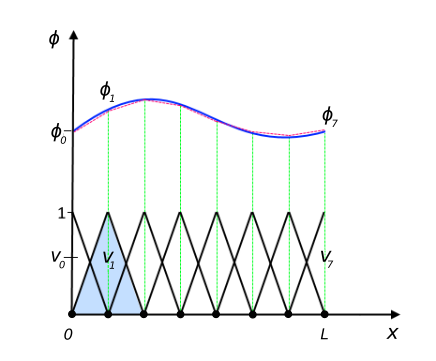
\includegraphics[width=\linewidth, trim= 0.5cm 0.5cm 0.5cm 0.5cm, clip]{figures/Ch2/plot-using-linear-combinations(1).png}
        \caption{}
        \label{fig:FEM_1Ddomain_uniform}
    \end{subfigure}
    \begin{subfigure}{0.5\textwidth}
        \centering
        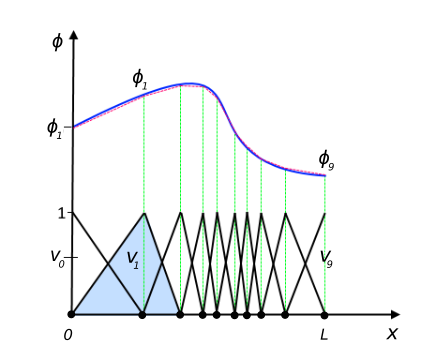
\includegraphics[width=\linewidth, trim= 0.5cm 0.5cm 0.5cm 0.5cm, clip]{figures/Ch2/plot-using-discretization(1).png}
        \caption{}
        \label{fig:FEM_1Ddomain_nonuniform}
    \end{subfigure}
    \caption{A one-dimensional domain is divided into segments (elements). The function $\phi$ is approximated to $\phi_h$ (marked in dashed red line) by linear combinations of linear basis functions $v_i$ (solid black lines). Nodes are marked as black dots. Figures (a) and (b) illustrates different distributions of the elements. Modified figure from \cite{FEM_comsol}.}
    \label{fig:FEM_1Ddomain}
\end{figure}

Equation (\ref{eq:FEM_difflikn_linearcomb}) discretizes the original problem (\ref{eq:FEM_difflikn}) into $N$ subdomains using linear combinations of basis functions. Figure \ref{fig:FEM_1Ddomain} illustrates this principle for a 1D problem. The solution domain $(0,L)$ is divided into small segments called \emph{finite elements}, and the joints between them are known as \emph{nodes}. An important feature of the basis functions is that they are non-zero only within the nearest neighbours of its respective node. Here, the basis function $v_i(x)$ has a value of 1 at node $i$, which decreases linearly to zero to the neighbouring nodes. The goal is to make the elements small enough so that the unknown solution over each element can be obtained by linear interpolation between the values of $\phi(x)$ at the two ends of the element. In other words, the denser the mesh, the closer the approximate solution will be to the physical solution.

Note that in figure \ref{fig:FEM_1Ddomain_uniform} the elements are uniformly distributed over the domain. This does not have to be the case, in figure \ref{fig:FEM_1Ddomain_nonuniform} more elements are concentrated in the region where the gradient of $\phi(x)$ is larger. An important advantage of FEM is that it offers great freedom in the selection of discretization. It is also worth mentioning that other interpolating functions may be chosen besides linear functions, depending on the problem at hand.

\subsection{Assembling the subdomains}
The next step in a FEM procedure is to combine all the local equations for all elements used for discretization. This process is known as \emph{assembly}. One major advantage of the FEM lies in its ability to define basis functions that are supported only over a small geometrical region. This implies that the integral in the left-hand side of equation (\ref{eq:FEM_mastereq_integral}) is zero everywhere except for the few regions where $v_i$ and $v_j$ overlap, and thus the system matrix $\mathbf{A}$ becomes sparse. With a very sparse system matrix the linear system can be generated and solved efficiently\cite{FEM_TheoryAndCompOfEM_Jian-Ming_Jin}. 

\begin{figure}[htb!]
    \begin{subfigure}{0.5\textwidth}
        \centering
        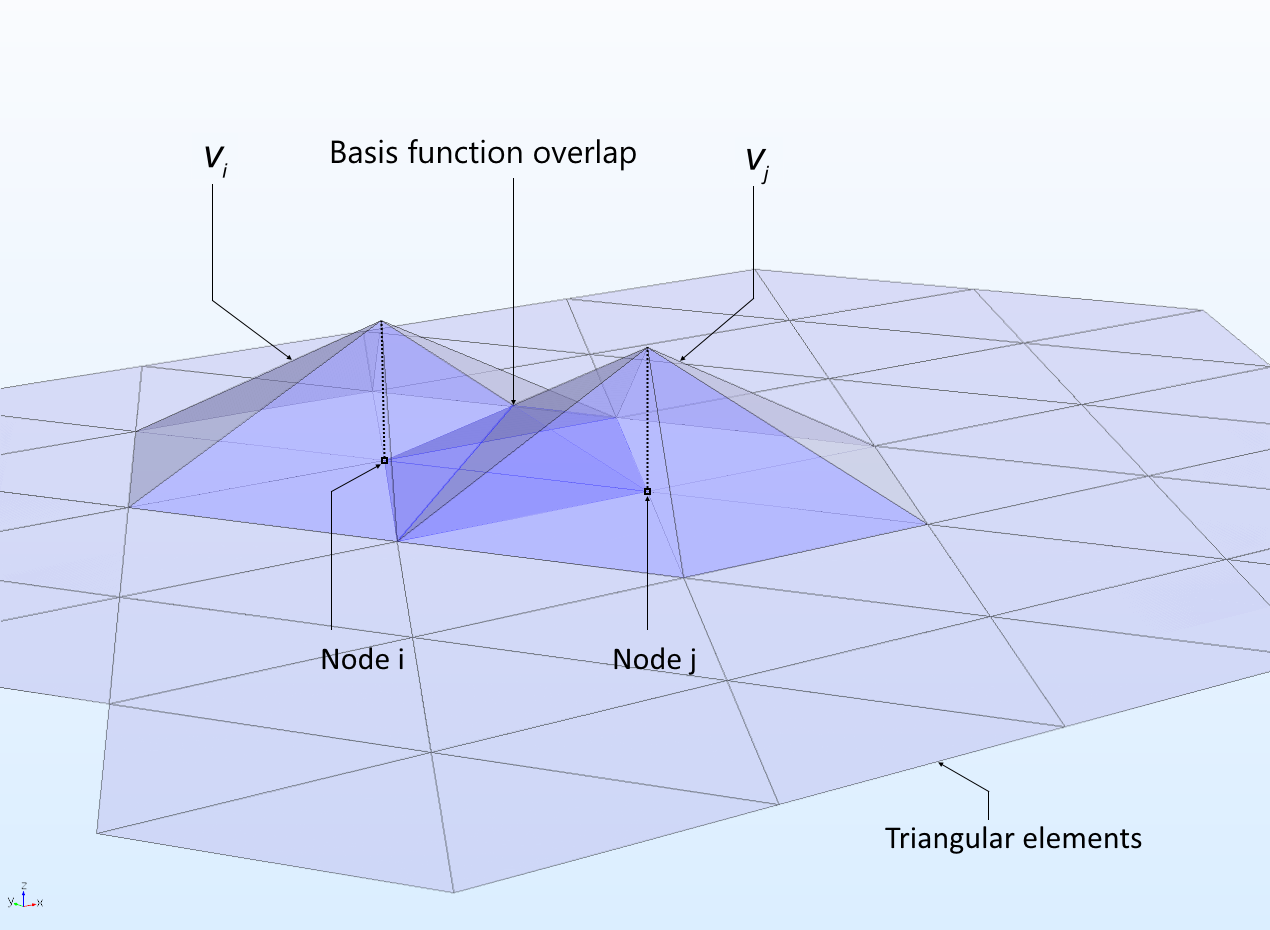
\includegraphics[width=\linewidth]{figures/Ch2/base-functions-overlap_fixed.png}
        \caption{}
        \label{fig:FEM_2Ddomain_overlap}
    \end{subfigure}
    \begin{subfigure}{0.5\textwidth}
        \centering
        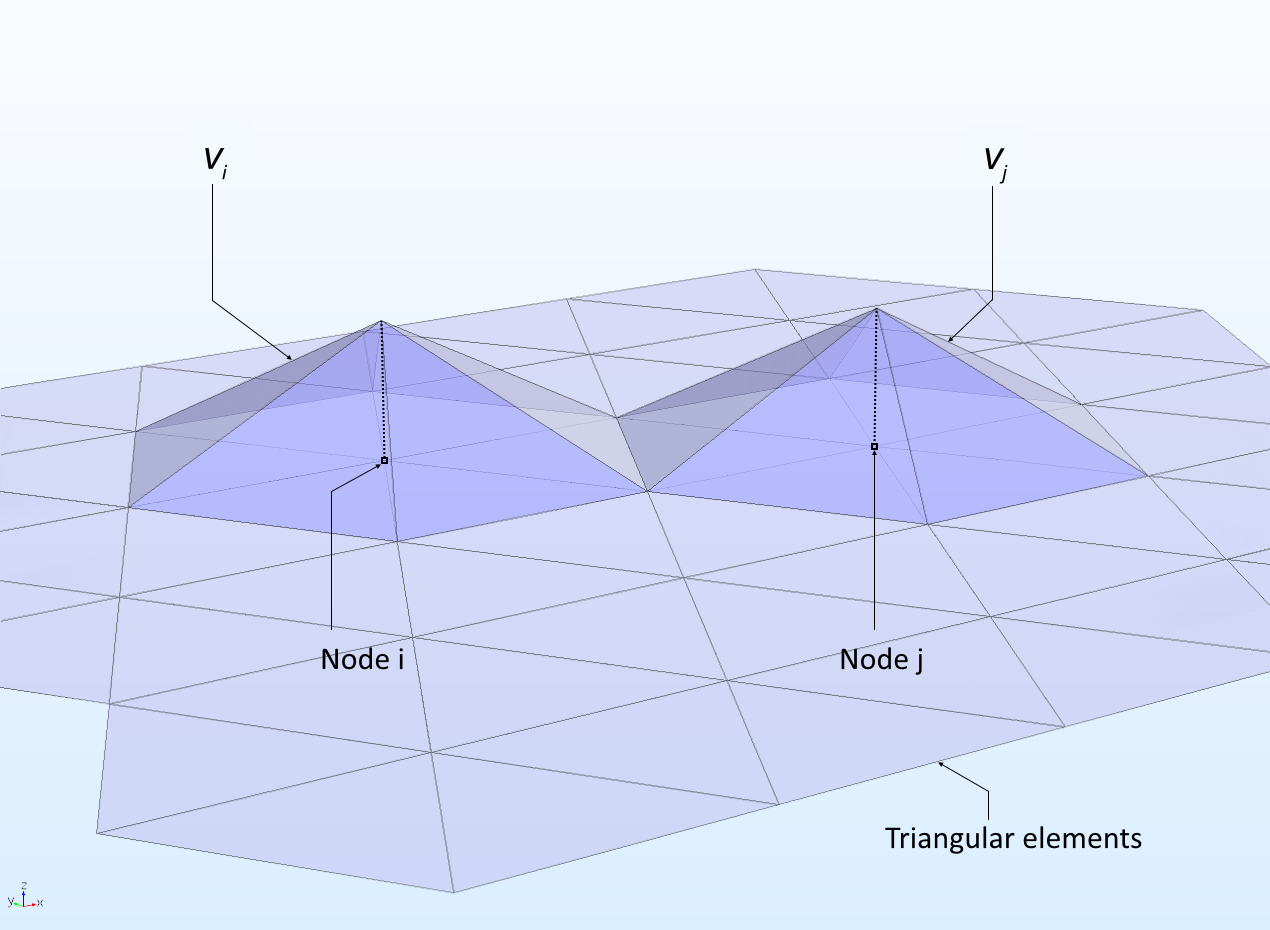
\includegraphics[width=\linewidth]{figures/Ch2/base-functions-no-overlap_fixed.png}
        \caption{}
        \label{fig:FEM_2Ddomain_nooverlap}
    \end{subfigure}
    \caption{A 2D domain discretized with triangular elements, basis functions $v$ have a value of 1 at the corresponding node and zero on all other nodes. (a) Two neighbouring nodes that share an element have overlapping basis functions. (b) Two basis functions that do not share elements and thus have no basis function overlap, although they do have a common element vertex. Edited figure from \cite{FEM_comsol}.}
    \label{fig:FEM_2Ddomain}
\end{figure}

Such basis functions are visualized in figure \ref{fig:FEM_2Ddomain} where a 2D domain is discretized into a triangular mesh with linear basis functions with a value of 1 at their respective nodes and zero on all other nodes. In figure \ref{fig:FEM_2Ddomain_overlap} two neighbouring nodes $i$ and $j$ are depicted. Their respective basis functions share two triangular elements and will thus have a non-zero contribution to the system matrix, as per equation (\ref{eq:FEM_mastereq_sum_Aji_bj}). If $i=j$ there is a complete overlap of the two basis functions. In figure \ref{fig:FEM_2Ddomain_nooverlap} the nodes are further apart and share no elements except having a common element vertex. When there is no overlap between $v_i$ and $v_j$ their contribution $A_{ij}$ to the system matrix is zero. Hence, in each row of $\mathbf{A}$ there will only be a few non-zero entries no matter how large the dimension of the matrix is. and the memory required to store the system matrix is thus proportional to $O(N)$\cite{FEM_TheoryAndCompOfEM_Jian-Ming_Jin}. After imposing boundary conditions to obtain the final form of the matrix equation (\ref{eq:FEM_mastereq_matrix}), it can be efficiently solved by linear solvers that exploit properties of sparse matrices\cite{FEM_TheoryAndCompOfEM_Jian-Ming_Jin}. FEM is therefore very suitable for large-scale applications with a large number of unknowns.

\subsection{Finite element analysis of vector fields}
The formulation of the finite element method so far is applicable to scalar fields. However, as all electrodynamic problems in three dimensions deal with vector electromagnetic fields, there is clear motivation to extend the formulation to include vector fields. This section will not go into details, but will rather mention the most important steps. The derivation is similar to section \ref{sec:FEM_generalprinciple}, but involves using vector basis functions which assigns degrees of freedom to the edges rather than to the nodes of the elements\cite{FEM_in_EM_jianming_jin}.%The finite element method described so far can be extended to deal with problems that involve vector fields. Such a formulation is important as all electrodynamic problems in three dimensions deal with vector electromagnetic fields. 

A typical electrodynamic problem involves finding the electric field $\mathbf{E}$ by solving Maxwell's equations (\ref{eq:ME}) subject to certain boundary conditions. The problem may be reduced to solving a single vector wave equation with well defined boundary conditions. As before, instead of solving these equations directly, a weak form solution may be sought by introducing vector weighting functions $\mathbf{W}_j$ and integrating over the entire domain $\Omega$. Discretization is obtained by first dividing the domain into small finite elements, typically triangular elements for a 2D domain and tetrahedral elements for a 3D domain. Within each element, $\mathbf{E}$ is interpolated using a set of discrete values. However, using the approach in section \ref{sec:FEM_generalprinciple} --- where the unknown field is assigned to a few points (nodes) on the element and then interpolated elsewhere using a set of scalar interpolation functions --- turns out to be very problematic; a series of difficulties arise when applying boundary conditions to the interpolated $\mathbf{E}$-field\cite{FEM_in_EM_jianming_jin}\cite{FEM_TheoryAndCompOfEM_Jian-Ming_Jin}. 



A better approach is to assign the tangential components of $\mathbf{E}$ along each edge of the element, $\mathbf{E}$ is then interpolated elsewhere by using a set of vector basis functions. For example, the field $\mathbf{E}^{(e)}$ in a triangular element $e$ can be interpolated as \cite{FEM_TheoryAndCompOfEM_Jian-Ming_Jin}
\begin{equation}
    \mathbf{E}^{(e)}(x,y) = \mathbf{V}_{12}^{(e)}(x,y)E_{12}^{(e)} + \mathbf{V}_{23}^{(e)}(x,y)E_{23}^{(e)} + \mathbf{V}_{31}^{(e)}(x,y)E_{31}^{(e)}
\end{equation}
where $E_{lk}^{(e)}$ denotes the tangential components of $\mathbf{E}$ at the edge that connects nodes $l$ and $k$ of element $e$, and $\mathbf{V}_{lk}^{(e)}$ is the corresponding interpolation or basis function. Figure \ref{fig:FEM_vector_element} illustrates the vector basis functions for element $e$. It is clear from the figures that the vector basis functions only have tangential components along their associated edge. They ensure tangential continuity of the interpolated field while allowing the normal component to be discontinuous\footnote{At the interface between two different media the elecromagnetic field is in general discontinuous. Specifically, the component of the displacement field $\mathbf{D}$ perpendicular to the boundary between media A and B is discontinuous in the amount $D_\text{A}^\perp-D_\text{B}^\perp=\sigma_f$, while the parallel component of the electric field $\mathbf{E}$ is continuous across the boundary, $E_\text{A}^\parallel - E_\text{B}^\parallel=0$.\cite{griffiths}}. Therefore, vector basis functions can be used to expand the vector field $\mathbf{E}$ accurately.
\begin{figure}[htb]
    \begin{subfigure}{0.32\textwidth}
        \centering
        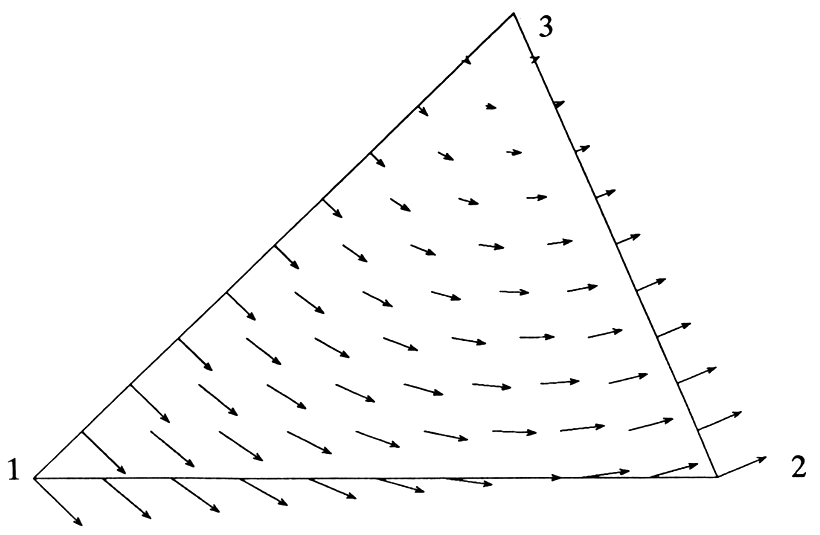
\includegraphics[width=\linewidth]{figures/Ch2/N1e_.png}
        \caption{}
    \end{subfigure}
    \begin{subfigure}{0.32\textwidth}
        \centering
        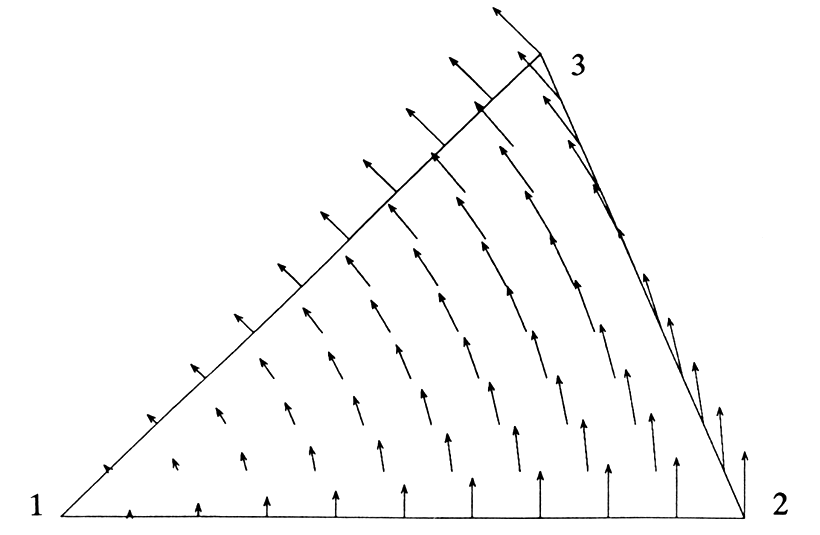
\includegraphics[width=\linewidth]{figures/Ch2/N2e_.png}
        \caption{}
    \end{subfigure}
    \begin{subfigure}{0.32\textwidth}
        \centering
        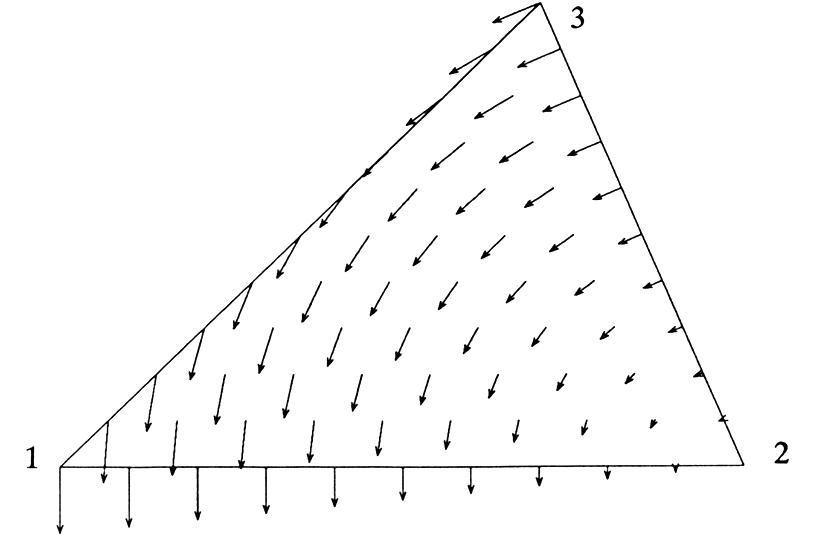
\includegraphics[width=\linewidth]{figures/Ch2/N3e_.png}
        \caption{}
    \end{subfigure}
    \caption{Vector basis functions for a triangular element $e$ with the nodes 1, 2 and 3. (a) $\mathbf{V}_{12}^{(e)}$, (b) $\mathbf{V}_{23}^{(e)}$, and (c) $\mathbf{V}_{31}^{(e)}$ are the vector basis functions assigned along their corresponding element edges. Figure from \cite{FEM_in_EM_jianming_jin}.}
    \label{fig:FEM_vector_element}
\end{figure}

When the electric field is interpolated in each element using tangential values at the element edges, the interpolated field $\mathbf{E}$ in the entire domain $\Omega$ can be expressed as 
\begin{equation}
    \mathbf{E} = \sum_{i=1}^{N_{\text{edge}}} \mathbf{V}_i E_i
    \label{eq:FEM_vector_sum}
\end{equation}
where $N_{\text{edge}}$ is the total number of edges, $E_i$ denotes the tangential component of $\mathbf{E}$ at the $i$th edge, and $\mathbf{V}_i$ is the corresponding vector basis function. A system matrix equation, a vector field equivalent to equation (\ref{eq:FEM_mastereq_matrix}), can then be found in a similar manner as in section \ref{sec:FEM_generalprinciple}; substituting equation (\ref{eq:FEM_vector_sum}) into the weak form solution of the wave equation and imposing the boundary conditions\cite{FEM_TheoryAndCompOfEM_Jian-Ming_Jin}.

This has been an attempt at a more simplified explanation of the finite element method, focusing more on intuitive understanding rather than gritty mathematics (while at the same time not ignoring it entirely). The assembly process to form the system of equations (\ref{eq:FEM_mastereq_matrix}), for example, is a much more intricate matter than presented, especially for vector fields.

%Assembly process similar to scalar fields method, but adds another connectivity array (in addition to element-$->$node), an element-to-edge array which describes the relation between the element numbers and edge numbers (see fig 9.13 in Jian-Ming Jin)

%%%%%%%%%%%%%%%%%%%%%%%%%%%%%%%%%%%%%%%%%%%%%%%%%%%%%%%%
\subsection{Domain truncation methods}
% http://math.mit.edu/~stevenj/18.369/pml.pdf
Electromagnetic problems often involve wave propagation in domains that extends to infinity. In numerical models this is usually overcome by truncating the computational domain to a finite domain, with external artificial boundaries that let waves pass through without any reflection. The most commonly used truncation techniques are the \emph{artificial} (or absorbing) \emph{boundary conditions} (\ac{abc}) and \emph{perfectly matched layers} (\ac{pml}). ABC techniques are more general than PML, however, PML can provide orders of magnitude lower reflections\cite{ABCandPML_Nataf}.

\subsubsection*{Scattering boundary condition}
A form of ABC are is the \emph{scattering boundary condition} (\ac{sbc}), which is an approximation of the Sommerfeld radiation condition. The Sommerfeld condition is one of the first transparent boundary conditions formulated for wave-type problems, and can be written for 2D fields as
\begin{equation}
    \lim_{r \to \infty}\sqrt{r}\left(\frac{\partial E_z}{\partial r}+ikE_z\right) = 0
    \label{eq:Sommerfeld_radiation_condition}
\end{equation}
when the EM wave is propagating in the xy-plane and the E-field is polarized in the z-direction. This condition is exactly non-reflecting when the boundary lies infinitely far away from the source. Obviously, the Sommefeld condition can not be applied exactly to a finite modeling domain so an approximation of equation (\ref{eq:Sommerfeld_radiation_condition}) must be made, 
\begin{equation}
    \mathbf{n}\cdot(\nabla E_z) + ikE_z = 0
\end{equation}
which is known as the first-order SBC\cite{PML_SBC_comsol}.


\begin{figure}[ht!]
    \centering
    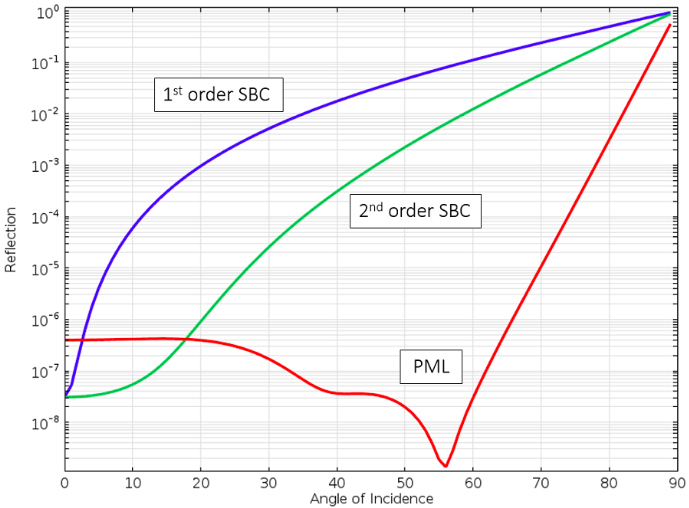
\includegraphics[width=0.7\linewidth]{figures/Ch2/PML_SBC_COMSOL.png}
    \caption{Reflection of a plane wave incident at the first- and second-order SBC, and PML boundaries with respect to angle of incidence. Figure from \cite{PML_SBC_comsol} where the data is from a FEM simulation using COMSOL Multiphysics.}
    \label{fig:PML_SBC}
\end{figure}

A significant limitation to SBC is that it is only perfectly transparent for scattered (outgoing) waves at normal incidence to the boundary\cite{comsol_referencemanual}. Second-order SBC is also possible which reduces reflection uniformly, see figure \ref{fig:PML_SBC}. However, there is still 10$\%$ reflection at an incidence angle of around 75$^\circ$.

\subsubsection*{Perfectly matched layers}
Perfectly matched layers were first introduced in 1994 by Berenger\cite{PML_Berenger} for use with Maxwell's equations. As the name suggests, PMLs are absorbing boundary \emph{layers} in contrast to absorbing boundary \emph{conditions} of ABC. The layer is an artificial anisotropic absorbing material placed adjacent to the edges of the grid, as depicted in figure \ref{fig:PML_region}. As a wave propagates through the absorbing layer it is exponentially decayed. Even if it reflects off the outer boundary, the returning wave will be exponentially tiny after one round trip. PML is special in that it does not reflect at the interface between the physical domain and the absorbing layer, whereas one would otherwise expect reflection in the transition from one material to another\cite{web:PML_MIT}.

\begin{figure}[htb]
    \centering
    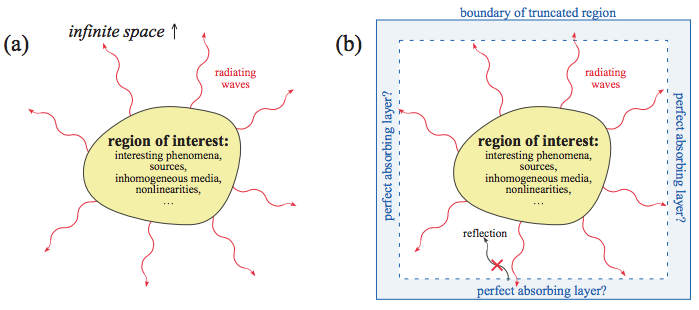
\includegraphics[width=0.9\linewidth]{figures/Ch2/PML_region.png}
    \caption{(a) A typical wave-equation problem; a region of interest where relevant phenomena are being investigated, from which some radiation escapes to infinity. (b) The same problem where space has been truncated to a finite computational domain. Absorbing layers are placed adjacent to the edges. A \emph{perfect} layer should absorb the outgoing waves without reflection from the edge of the absorber. Figure from \cite{web:PML_MIT}.}
    \label{fig:PML_region}
\end{figure}

The original formulation by Berenger\cite{PML_Berenger} was based on splitting the EM wave solutions into a sum of two artificial fields inside the PML region. Later, it was found that the PML could be derived from a modified form of Maxwell's equations based on stretched coordinates\cite{PML_coordstretch}. This complex-coordinate approach is essentially based on analytic continuation of Maxwell's equations into complex spatial coordinates where the fields are exponentially decaying\cite{web:PML_MIT}. In implementing PML to the finite element method, the preferred approach is to consider the PML as an anisotropic medium, a derivation can be found in \cite{FEM_TheoryAndCompOfEM_Jian-Ming_Jin}.

PML is perfectly reflectionless only when solving the exact wave equations. As soon as the problem is discretized (as in FEM) to an approximate wave equation, the analytical perfection of PML is no longer valid. The PML is still an absorbing material; the discrete waves within the layer are still being attenuated. However, the boundary between the PML and the regular medium is no longer reflectionless, but these reflections are small as long as the discretization is a good approximation of the exact wave equation\cite{web:PML_MIT}. To further minimize this reflection it is desirable to use a mesh in the PML that aligns with the anisotropy in the material properties\cite{PML_SBC_comsol}. In figure \ref{fig:PML_mesh} the appropriate PML meshes are shown for 2D circular and 3D spherical domains, with 5 layers uniformly distributed. \text{\color{red}}

\begin{figure}[htb]
    \centering
    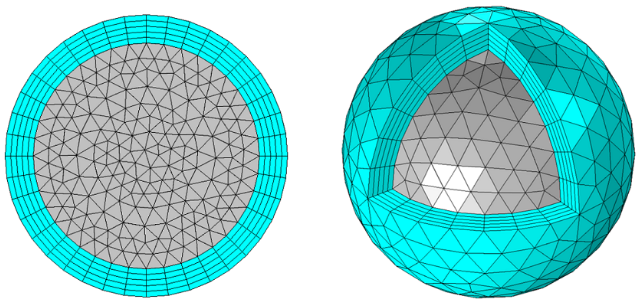
\includegraphics[width=0.6\linewidth]{figures/Ch2/PML_mesh.png}
    \caption{Appropriate meshes for 2D and 3D spherical PMLs. Figure from \cite{PML_SBC_comsol}.}
    \label{fig:PML_mesh}
\end{figure}

In figure \ref{fig:PML_SBC} a plane wave is incident on either a SBC or a PML boundary, modelled in the FEM software COMSOL Multiphysics\cite{PML_SBC_comsol}. The PML reflects the least amount across the widest range, however, there is still reflection when the incident wave is almost parallel to the boundary. A major advantage of PML over ABC in general, is that their absorbing performance can be improved systematically by simply increasing the number of layers\cite{FEM_TheoryAndCompOfEM_Jian-Ming_Jin}. The flexibility of FEM also permits the use of non-rectangular PMLs.

It is worth to note that PMLs do not absorb evanescent solutions to the wave equation\cite{PML_reflectionOfEvanescentWaves1}\cite{PML_reflectionOfEvanescentWaves2}. Numerical
reflection observed in wave-structure interaction problems may therefore be interpreted as the reflection of evanescent fields surrounding the structures\cite{PML_reflectionOfEvanescentWaves2}. A simple fix is to make sure the computational domain large enough so that the evanescent waves decay before hitting the boundary.


%\cleardoublepage